\documentclass[10pt,a4paper]{article}
\usepackage{graphicx}
\usepackage[utf8]{inputenc}
\usepackage{subfig}
\graphicspath{ {./images/} }

%%%%%%%%%%%%%%%%%%%%%%%%%%%
% MODIFY:

\newcommand{\authorA}{Jia Long Ji Qiu}
\newcommand{\authorB}{Jiabo Wang}
\newcommand{\authorC}{Yilun Liu}
\newcommand{\groupNumber}{J} % - YOUR GROUP NUMBER
\newcommand{\exerciseNumber}{1} % - THE NUMBER OF THE EXERCISE
\newcommand{\sourceCodeLink}{https://github.com/jialongjq/mlcms}

\newcommand{\workPerAuthor}{
\authorA&Task 1&1/3\%\\
      &Task 2&1/3\%\\
      &Task 3&1/3\%\\
      &Task 4&1/3\%\\
      &Task 5&1/3\%\\
      \hline
\authorB&Task 1&1/3\%\\
      &Task 2&1/3\%\\
      &Task 3&1/3\%\\
      &Task 4&1/3\%\\
      &Task 5&1/3\%\\
      \hline
\authorC&Task 1&1/3\%\\
      &Task 2&1/3\%\\
      &Task 3&1/3\%\\
      &Task 4&1/3\%\\
      &Task 5&1/3\%\\
}

%%%%%%%%%%%%%%%%%%%%%%%%%%%

%%
% imports for the exercise sheets
%

\usepackage[utf8]{inputenc}
\usepackage{amsmath}
\usepackage{amsfonts}
\usepackage{amssymb}

\usepackage[yyyymmdd]{datetime}
\renewcommand{\dateseparator}{--}

\usepackage[left=2cm,right=2cm,top=3cm,bottom=3cm]{geometry}
\usepackage{listings, xcolor}

\definecolor{codegreen}{rgb}{0,0.6,0}
\definecolor{codegray}{rgb}{0.5,0.5,0.5}
\definecolor{codepurple}{rgb}{0.58,0,0.82}
\definecolor{backcolour}{rgb}{0.95,0.95,0.92}

\lstdefinestyle{mystyle}{
    backgroundcolor=\color{backcolour},   
    commentstyle=\color{codegreen},
    keywordstyle=\color{magenta},
    numberstyle=\tiny\color{codegray},
    stringstyle=\color{codepurple},
    basicstyle=\ttfamily\footnotesize,
    breakatwhitespace=false,         
    breaklines=true,                 
    captionpos=b,                    
    keepspaces=true,               
    showspaces=false,                
    showstringspaces=false,
    showtabs=false,                  
    tabsize=2
}

\lstset{style=mystyle}

\usepackage{hyperref}

\usepackage{amsthm}
\newtheorem{lem}{Lemma}
\newtheorem{thm}{Theorem}
\newtheorem{cor}{Corollary}
\newtheorem{rem}{Remark}
\newtheorem{definition}{Definition}
\newtheorem{ter}{Terminology}

\usepackage{graphicx}

\newcommand{\M}{\mathcal{M}}
\newcommand{\N}{\mathcal{N}}
\newcommand{\K}{\mathcal{K}}
\newcommand{\SPDk}{\mathbb{P}^k}
\newcommand{\vol}{\text{vol}}

\newcommand{\Figref}[1]{Figure~\ref{#1}}
\newcommand{\figref}[1]{figure~\ref{#1}}
\newcommand{\Eqnref}[1]{Equation~(\eqref{#1})}
\newcommand{\eqnref}[1]{equation~(\eqref{#1})}

\usepackage{float}
\usepackage{tabularx}

\usepackage{fancyhdr}
\pagestyle{fancy}

\usepackage{totcount}
\newtotcounter{taskCounter}
\newtotcounter{pointCounter}
\newenvironment{task}[1]{\noindent\stepcounter{taskCounter}\textbf{Report on task #1}\smallbreak\hrule\smallbreak}{\smallbreak\hrule\bigbreak}

\usepackage{array}

\usepackage{caption}
\usepackage{subcaption}

\title{Report for exercise \exerciseNumber~from group~\groupNumber}

\makeatletter
\let\thetitle\@title
\let\theauthor\@author
\let\thedate\@date
\makeatother

\providecommand{\versiondate}{\today}

\lhead{Exercise sheet \exerciseNumber}
\chead{Master Praktikum: Modelling and Simulation of Crowds WS2022/23}
\rhead{TUM}
\lfoot{Report of Group \groupNumber}
\cfoot{\thepage}
\rfoot{Last compiled: \versiondate}
\renewcommand{\headrulewidth}{0.4pt}
\renewcommand{\footrulewidth}{0.4pt}

\newcommand{\frontpage}{
\begin{center}
\textbf{\thetitle}\\~\\
\end{center}
\begin{table}[H]
\begin{tabular}{ll}
Tasks addressed:&\total{taskCounter}\\
Authors:&\authorA\\
&\authorB\\
&\authorC\\
Last compiled:&\versiondate\\
Source code:&\sourceCodeLink
\end{tabular}
\end{table}
\vfill
The work on tasks was divided in the following way:
\begin{table}[H]
\begin{tabularx}{\textwidth}{X|p{2cm}|p{2cm}}
\workPerAuthor
\end{tabularx}
\end{table}
\newpage
}

\begin{document}

\frontpage

\begin{task}{1, Setting up the modeling environment}
\noindent\textbf{High level description:} Firstly, a graphical visualization environment was set up. It consists in an empty grid and a set buttons on its left side (Figure \ref{fig1}). The project is implemented in Python and the \textbf{tkinter} package was used for the graphical aspects.

\begin{figure}[h]
    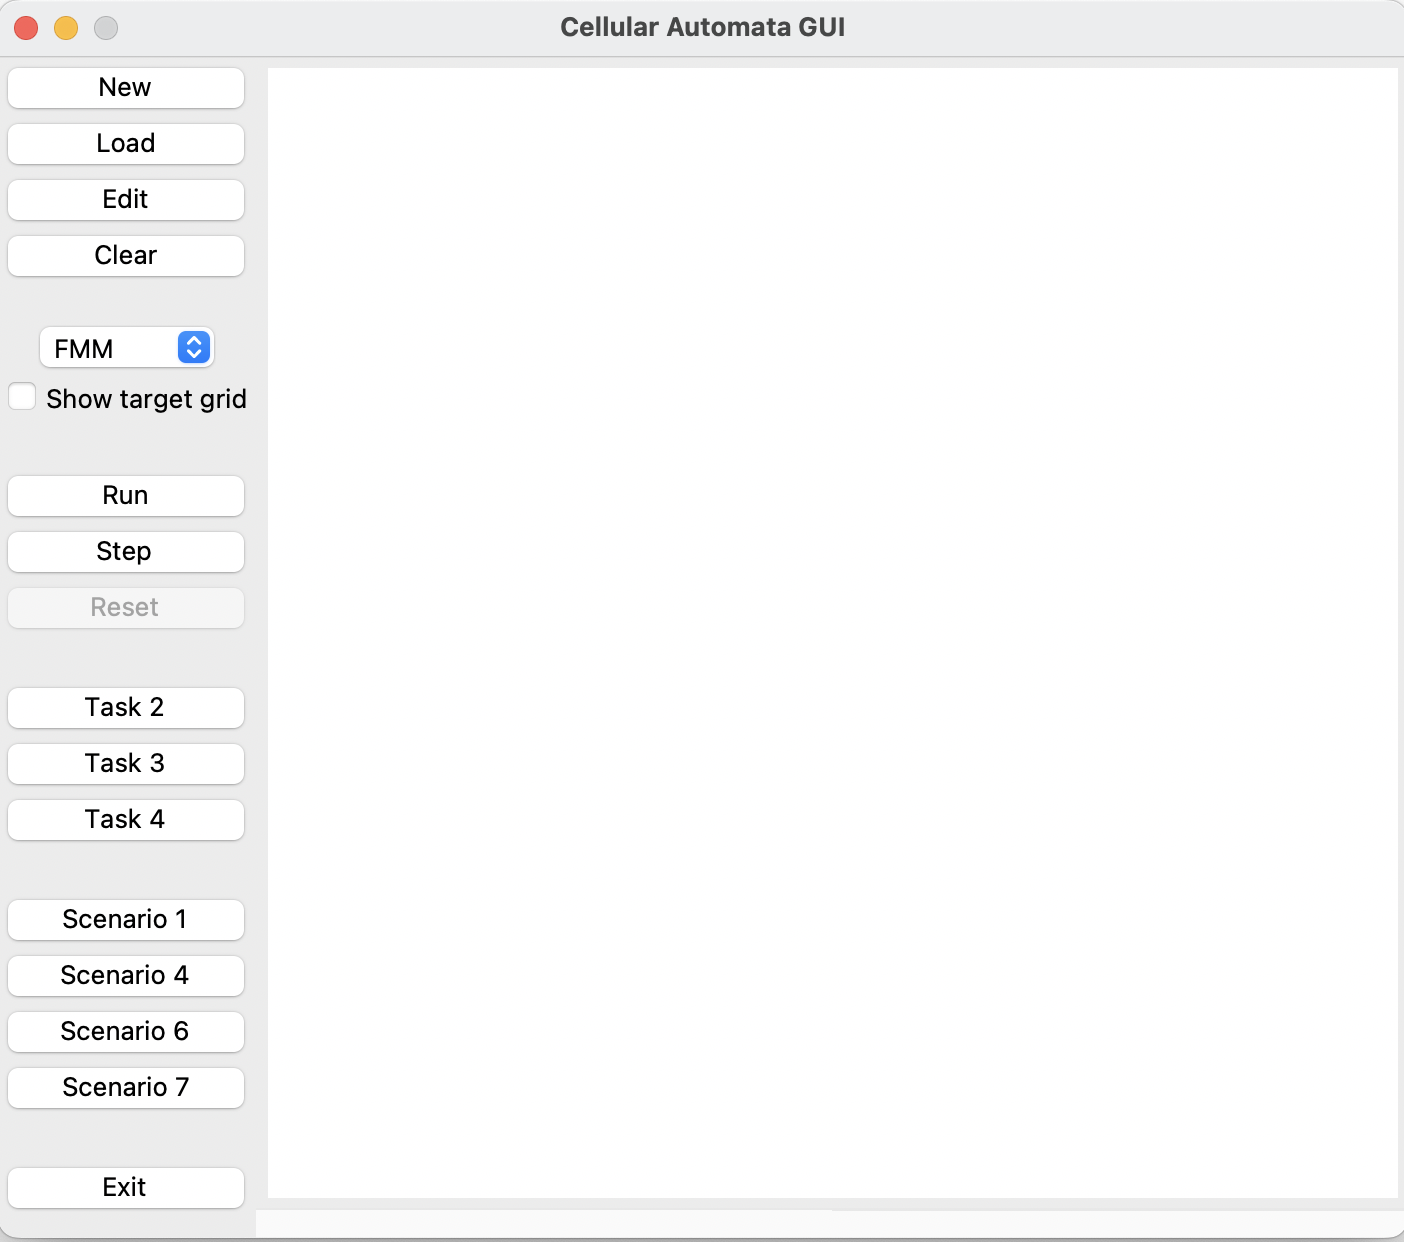
\includegraphics[width=10cm]{menu}
    \centering
    \caption{Empty grid with the set of buttons on the left side}
    \label{fig1}
\end{figure}

The function of the first button \textbf{New} is to allow the user to set up the dimensions of the scenario (width and length) as we can see in the figure \ref{fig2}.
\begin{figure}[h]
    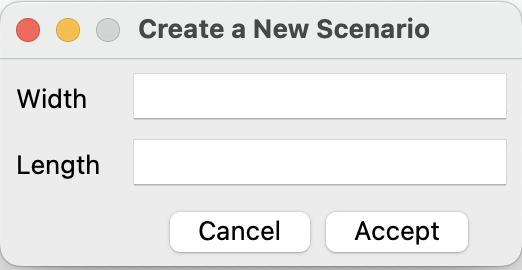
\includegraphics[width=5cm]{new}
    \centering
    \caption{New button window}
    \label{fig2}
\end{figure}

The next button is \textbf{Load} and it allows the user to load a .json file (see an example in figure \ref{fig3}) with personalized scenarios. In this file, it has to be specified the dimensions of the scenario and the positions of the pedestrians, obstacles and targets (obviously inside in the dimensions of the scenario).

\begin{figure}[h]
    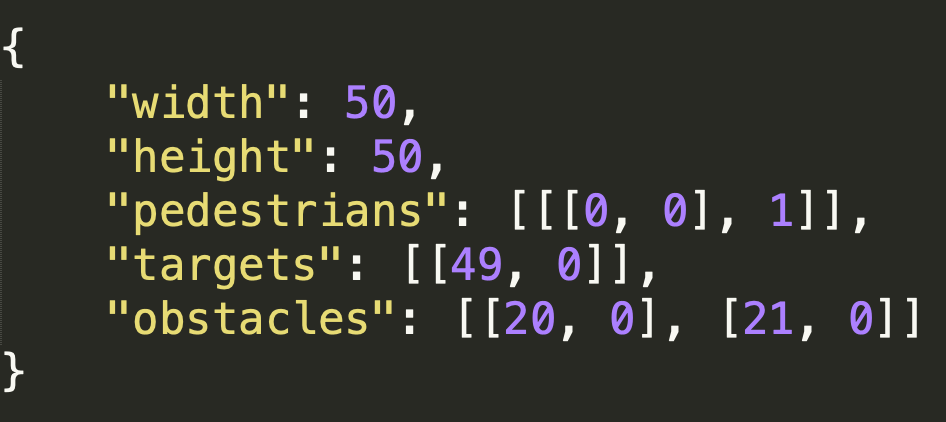
\includegraphics[width=5cm]{json}
    \centering
    \caption{Example of a .json file}
    \label{fig3}
\end{figure}

\hfill \break 

The button \textbf{Edit} allows the user to make an edit of the scenario: it is possible to add or remove pedestrians, targets and obstacles. It has to be specified the position of the objects and in the case of adding pedestrians, it also needs the desired speed that will acquire the pedestrian.

\begin{figure}[h]
    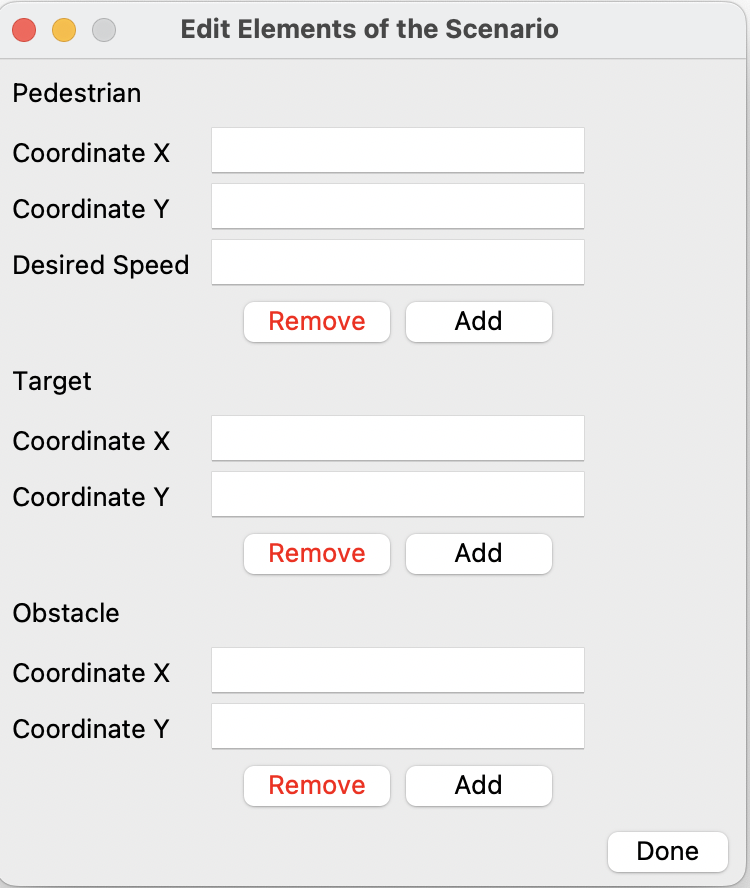
\includegraphics[width=6cm]{edit}
    \centering
    \caption{Edit window}
    \label{fig4}
\end{figure}

In the next position we have the button \textbf{Clear} its function is to make ride of all the elements that are in the scenario in that moment: it includes pedestrians, obstacles and targets.

Next there is an \textbf{Option Menu} (shown in the figure \ref{fig5}) that allows the user to choose among three different algorithms (FMM, Dijkstra and Basic) that will be used for the computation of distances.  

\begin{figure}[h]
    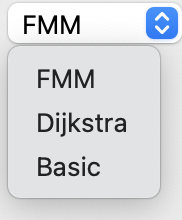
\includegraphics[width=3cm]{option menu}
    \centering
    \caption{Algorithms Option Menu}
    \label{fig5}
\end{figure}

Below the option menu, there is a \textbf{Check Button} that allows the user to alternate between the normal (figure \ref{fig6}) and target grid distance-based (figure \ref{fig7}) views: 

\begin{figure}[!h]
    \begin{minipage}[c]{0.4\linewidth}
        \centering
        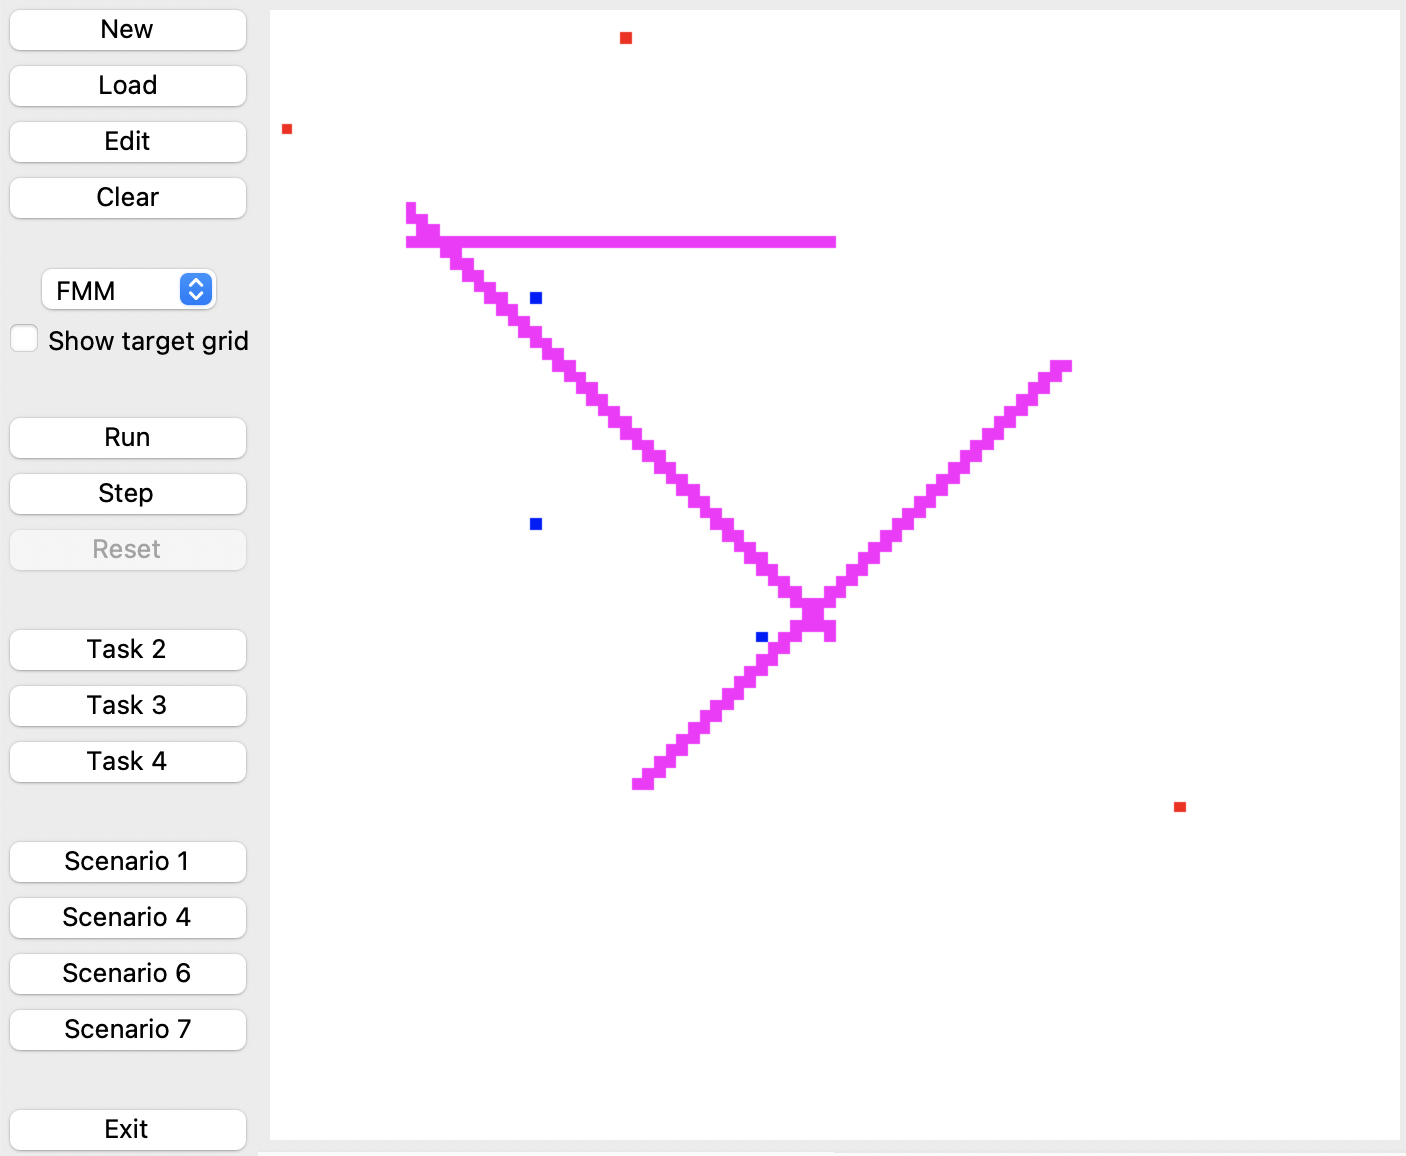
\includegraphics[width=5cm]{normal_view}
        \caption{Normal View of the scenario}
        \label{fig6}
    \end{minipage}\hfill
    \begin{minipage}[c]{0.4\linewidth}
        \centering
        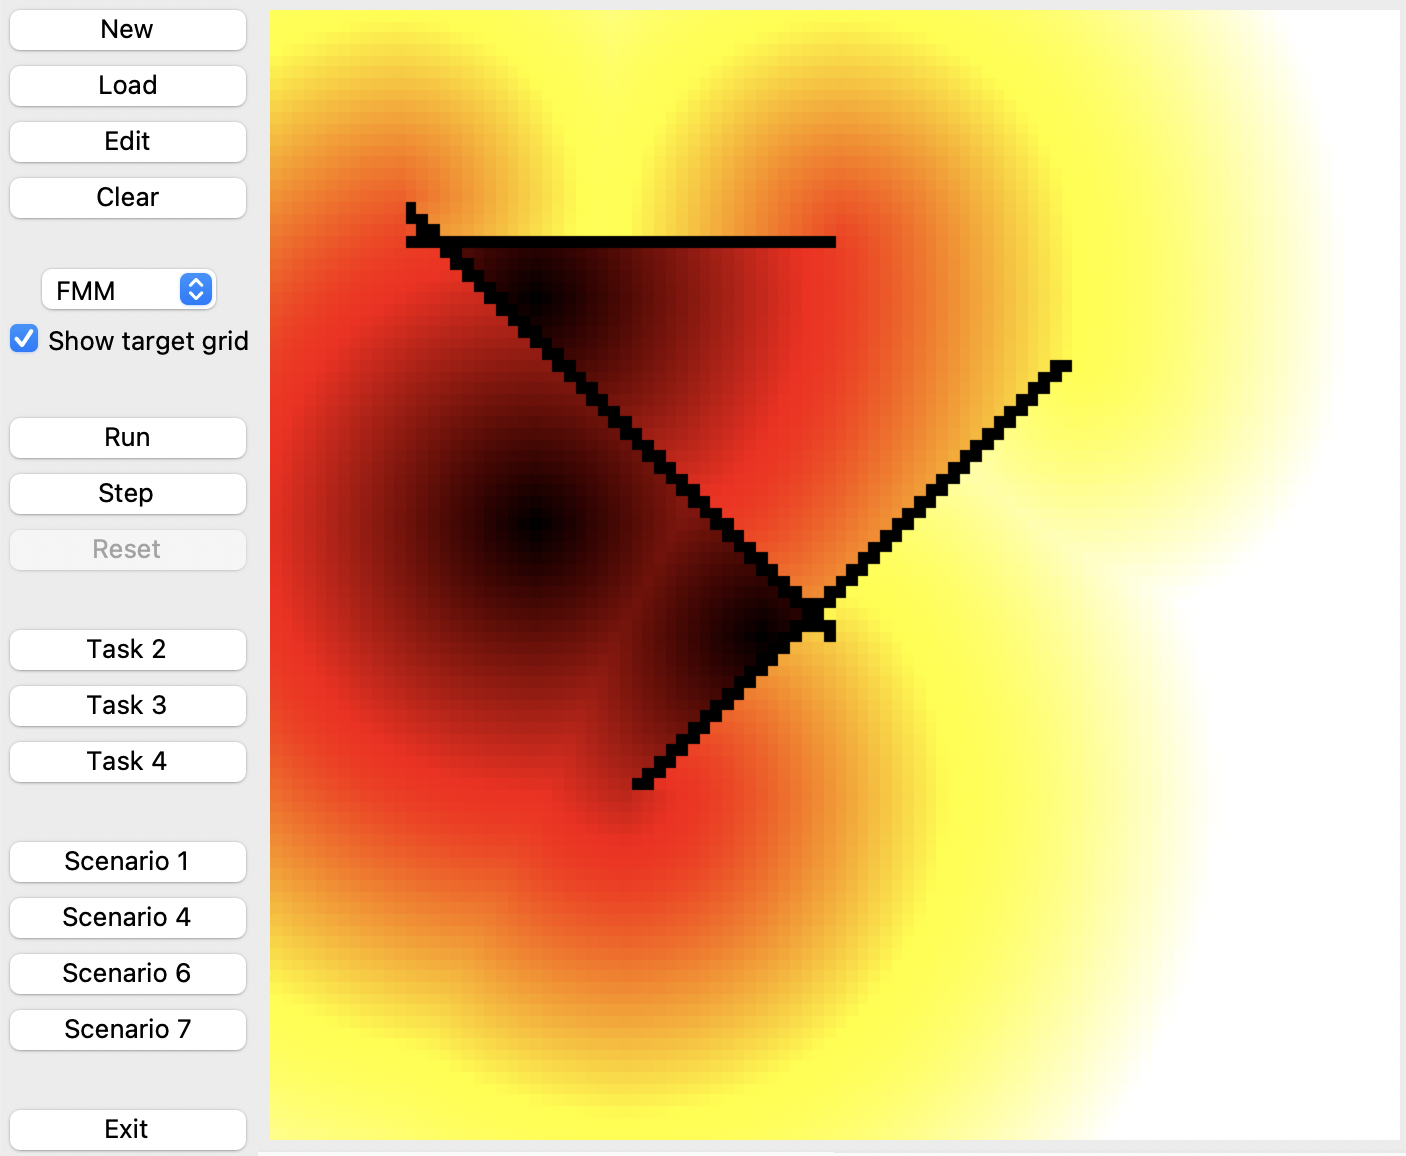
\includegraphics[width=5cm]{special_view}
        \caption{Grid Distance View of the scenario}
        \label{fig7}
    \end{minipage}
\end{figure}

The next button is \textbf{Run} and its function is to run a simulation of the defined scenario, that is the pedestrian tries to reach the nearest target in the quickest way and avoiding the obstacles.

The button located below is \textbf{Step} and its function is similar of the \textbf{Run}, but in this case, it only allows the pedestrian to one only movement. A defined can be simulated by one click with \textbf{Run} or just clicking the \textbf{Step} until all pedestrians reach a target or cannot move.

The following button is the \textbf{Restart} button that allows the user to restart the scenario back to the one defined just before running a simulation or making the first step. At the beginning it is disabled and it will just be enable after making a run or a step.

The next buttons \textbf{Task 2, Task 3, Task 4, Scenario 1, Scenario 4, Scenario 6, Scenario 7} represents the different scenarios required in the statement. Once clicked the button, it will draw the scenario and by clicking \textbf{Run} it will simulate the scenario.

\begin{figure}[h]
    
\includegraphics[width=3cm]{density}
    \centering
    \caption{Density Option Menu for the scenario 4}
    \label{density}
\end{figure}

The Option Menu \textbf{Density} is to select the different density of pedestrians per square meters for the scenario 4, the options are: 0.5, 1, 2, 3, 4, 5, 6.

Finally, we have the \textbf{Exit} button that closes the GUI.\\
\textbf{Code and Implementation} The project is implemented in \textbf{Python} (vers. 3.9.13) and \textbf{tkinter} (vers. 8.6). The two main objects are: Scenario and Pedestrian.

The most important attributes of \textbf{Scenario} are:

\begin{itemize}
    \item pedestrians: a list containing all the \textbf{Pedestrian} objects
    \item grid: a numpy array that contains the information of every cell of the scenario, indicating if there is a Pedestrian, a target, an obstacle or it is empty. A pedestrian is represented with the color red, a target is represented with blue and an obstacle is represented as magenta
    \item target\_distance\_grid: recomputes the target distances from every cell with the specified algorithm 
\end{itemize}

The class \textbf{Pedestrian} contains information such as the position and his speed. The main method of the class is:
\begin{itemize}
    \item update\_step: moves to the cell with the lowest distance to the target
\end{itemize}

The pedestrians are be able to move during a \textbf{simulation} because the steps that a pedestrian has to do is based on a basic algorithm that consists of calculating all the distances that each cell of the scenario is to the targets and store the minimum one (that is the nearest target). Then the pedestrian just has to choose among his neighbors cells the one that has the lowest distance to a target and move to it. 

\end{task}

\pagebreak

\begin{task}{2, First step of a single pedestrian}
Task 2 consists in defining a scenario with 50 by 50 cells (2500 in total), a single pedestrian at position (5, 25) and a target 20 cells away from them at (25, 25). \\
This scenario can be executed in our cellular automaton step by step or in one fell swoop with the \textbf{Run} button. Each cell is 1m x 1m, and the speed of the pedestrian is 1 m/step. After simulating this scenario, the pedestrian reaches the target after 20 steps and waits here in the remaining 5 steps.

\begin{figure} [!h]
 \centering
  \subfloat[Initial setup of the scenario]{
   \label{1}
    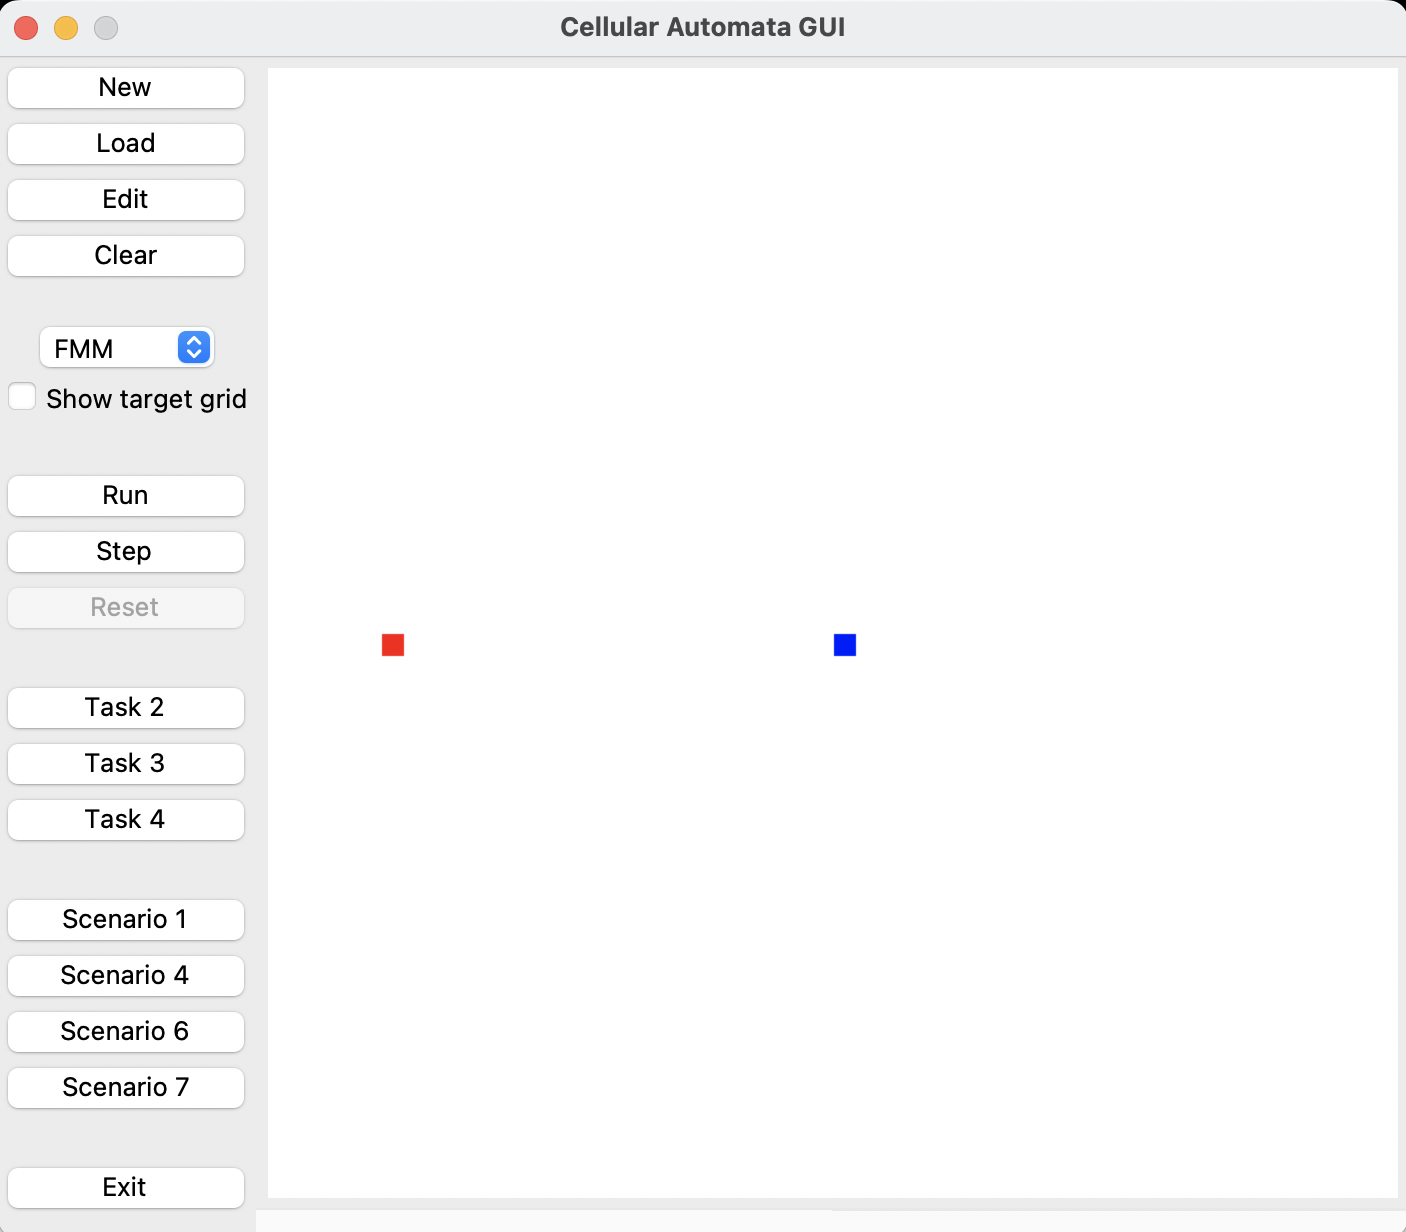
\includegraphics[width=0.3\textwidth]{task2_1}}
  \subfloat[In the middle of the simulation]{
   \label{2}
    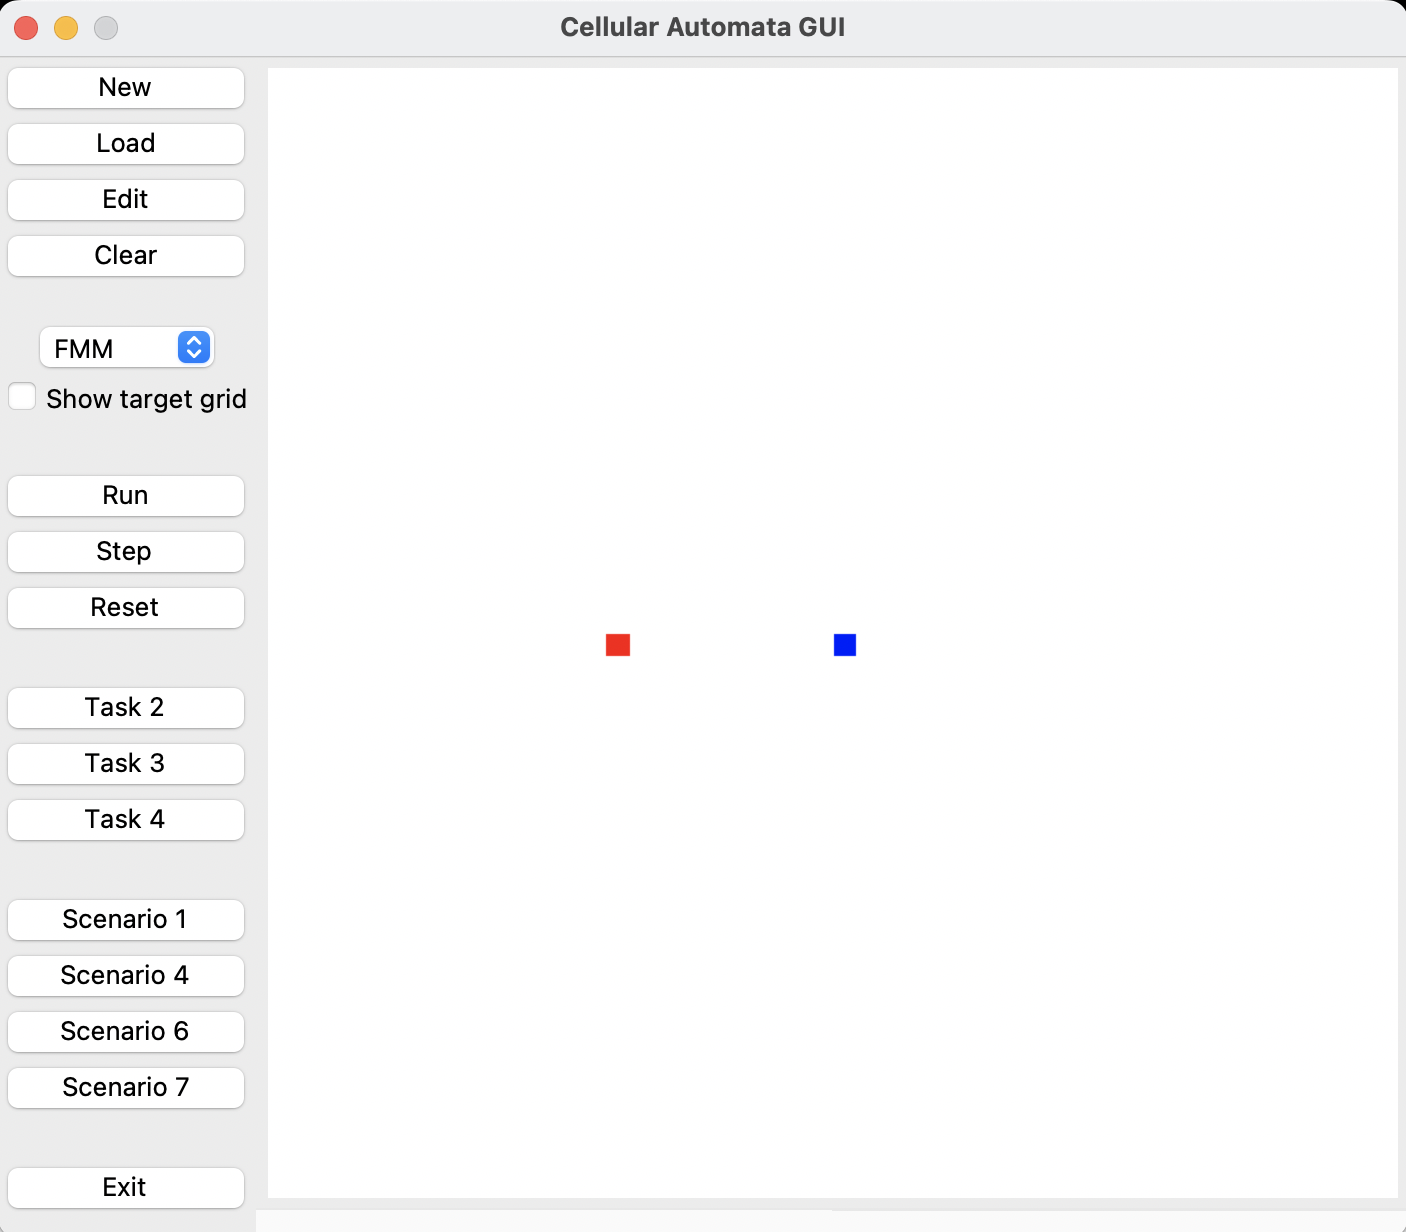
\includegraphics[width=0.3\textwidth]{task2_2}}
  \subfloat[End of the simulation]{
   \label{3}
    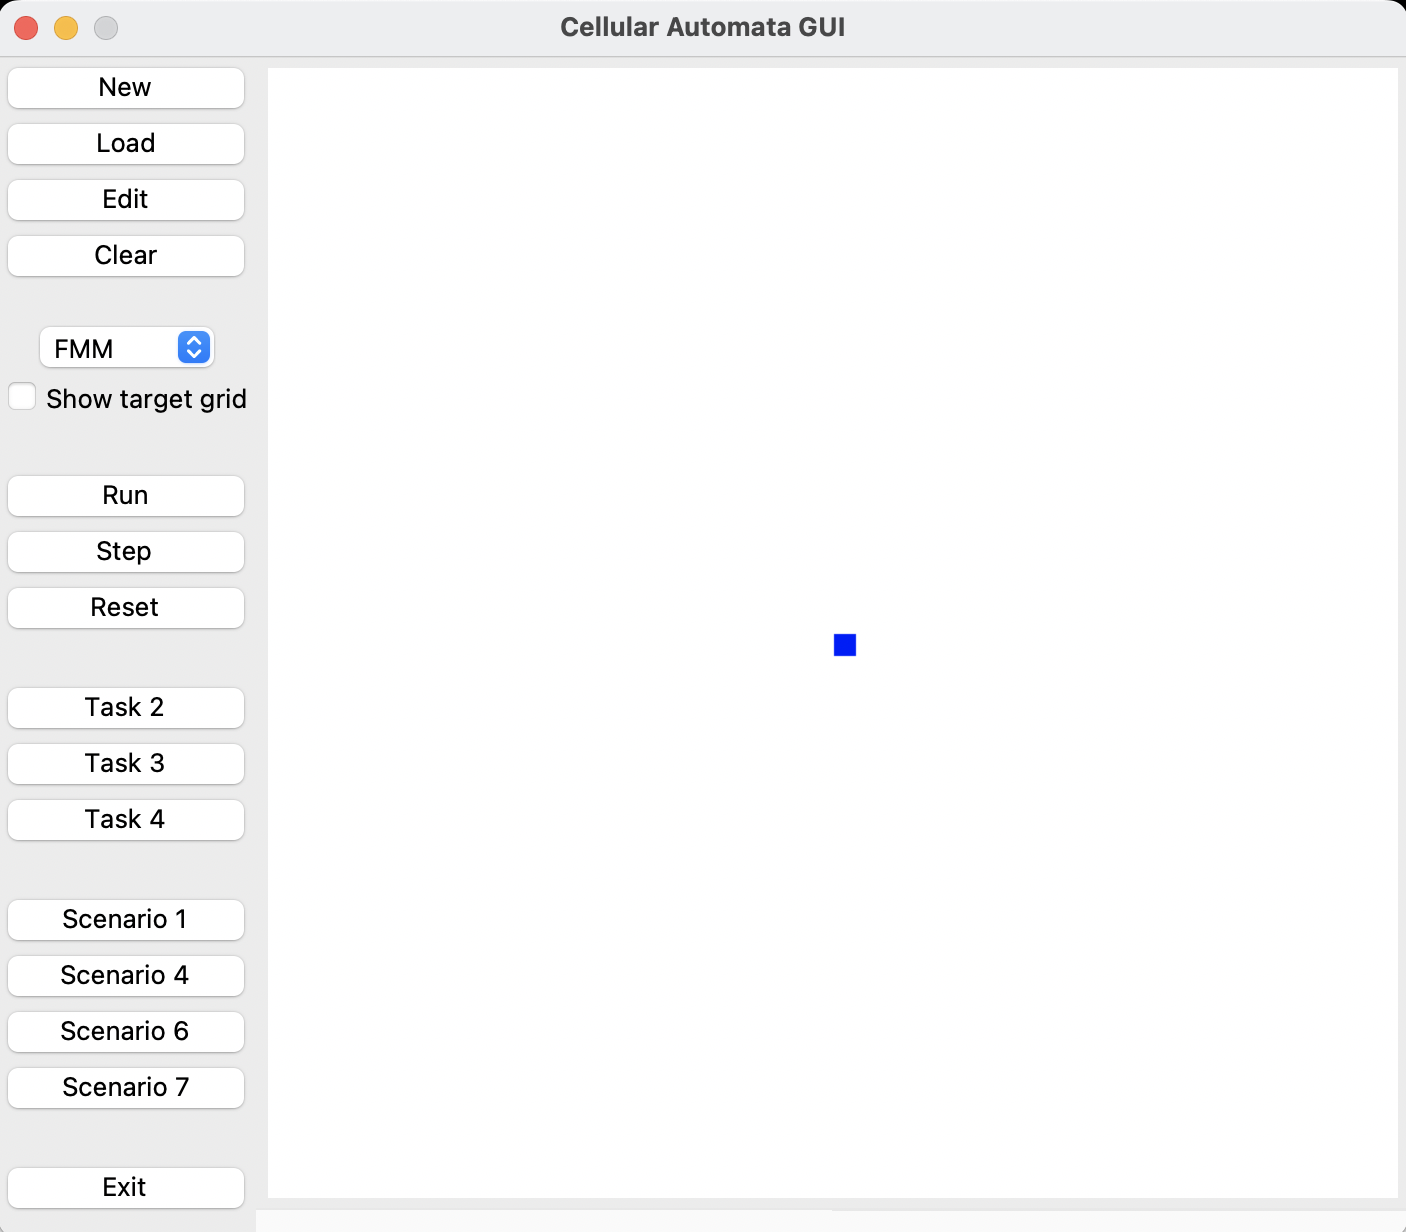
\includegraphics[width=0.3\textwidth]{task2_3}}
 \caption{Screenshoots showing the different stages of the simulation}
 \label{f}
\end{figure}

\end{task}

\pagebreak

\begin{task}{3, Interaction of pedestrians}
This task consists in placing five pedestrians equally spaced on a circle in the same distance around a single target in the center of the scenario (Figure \ref{1a}), with the objective of showing that they can reach the target at the same time with the same walking speed.

Before this task, the notion of ``walking speed" was not introduced yet, so the movement the pedestrians did consisted only in continuously selecting the neighbor cell with the minimum distance to reach the target, without taking into account the speed neither the obstacles. For this reason, the implementation of the walking speed should be explained first.

The walking speed has been defined as ``the distance a pedestrian can travel in one tick", where each tick is an execution of a single step. For example, considering the Euclidean distance between cells, if a pedestrian is placed at the position (0, 0) and has a walking speed of 1, it will take 2 ticks to reach the position (0, 2), whereas with a walking speed of 2 it would only take 1 tick.

However, since both the speed and the distance can be positive real numbers, it is not as simple as just moving through the same number of cells in each iteration. Instead, the real distance traveled during one step must be kept in track, so that the remaining distance can be saved for the next one. For example, a pedestrian with a walking speed of 1.5 placed at the position (0, 0), in order to reach the position (0, 3), it should move to (0, 1) in the first tick, save a remaining distance of 0.5 for the next tick, and move from (0, 1) to (0, 3) in the second tick since the available distance to travel will be 2. The same goes for diagonal movements, since two cells placed diagonally have a distance of $\sqrt{2}$, if a pedestrian with a walking speed of 1 placed at the position (0, 0) has to reach the position (2, 2) by only making diagonal movements, it should not move during the first tick, save a distance of 1 for the next tick, move to (1, 1) in the second tick, save $2-\sqrt{2}$ for the next tick and move to (2, 2) in the third tick, since the accumulated distance $1+2-\sqrt{2}$ will be greater than $\sqrt{2}$. This way, the real walking speed in a simulation will be close to the desired speed in the long run. A pseudo-code of this algorithm is described in Algorithm \ref{alg:update_step}

\begin{algorithm}[H]
	\caption{Update Step} 
	\label{alg:update_step}
	\begin{algorithmic}[1]
	    \State available distance = movement speed + accumulated distance
	    \State accumulated distance = 0
		\While {available distance $>$ 0}
		    \State next cell distance = distance in current position
		    \State next position = current position
			\For {each position of the unoccupied neighbors}
				\State \textbf{if} {distance to target in neighbor position $<$ next cell distance} \textbf{then}
				\State \hspace{4mm} update next position and next cell distance to the corresponding neighbor position
                \State \textbf{else if} distance to target in neighbor position $==$ next cell distance \textbf{then}
                \State \hspace{4mm} keep the position with shorter walking distance
			\EndFor
			\State \textbf{if} next position $\neq$ current position \textbf{then}
			    \State \hspace{4mm} distance to travel = Euclidean distance from current position to next position
			    \State \hspace{4mm} \textbf{if} distance to travel $\leq$ available distance \textbf{then}
			        \State \hspace{8mm} subtract the distance to travel to the
			        available distance
			        \State \hspace{8mm} move to the next position
			    \State \hspace{4mm} \textbf{else} empty the available distance and save it in accumulated distance
			\State \textbf{else} break
		\EndWhile
	\end{algorithmic} 
\end{algorithm}

Now, proceeding to the simulation, the scenario dimensions are 50 x 50, so the target is placed in the position (24, 24) and the five pedestrians are placed as follows:
\begin{itemize}
    \item pedestrian 1: ((0, 6), 1)
    \item pedestrian 2: ((0, 42), 1)
    \item pedestrian 3: ((6, 0), 1)
    \item pedestrian 4: ((48, 6), 1)
    \item pedestrian 5: ((48, 42), 1)
\end{itemize}

All pedestrians are located in an Euclidean distance of 30 units from the target and all of them have the same walking speed, so that all of them can reach at the same time the target.

As in the previous task, this task can be simulated step by step or in one fell swoop with the \textbf{Run} button. Figure  shows the different stages of the simulation. The goal of the task is that all the pedestrians reach the target, so the target have been made to be "absorbing" (Figure \ref{3a}). 

After simulating the scenario defined previously, all the pedestrians reach the target roughly at the same time because they are at the same distance.

\begin{figure} [!h]
 \centering
  \subfloat[Initial setup of the scenario]{
   \label{1a}
    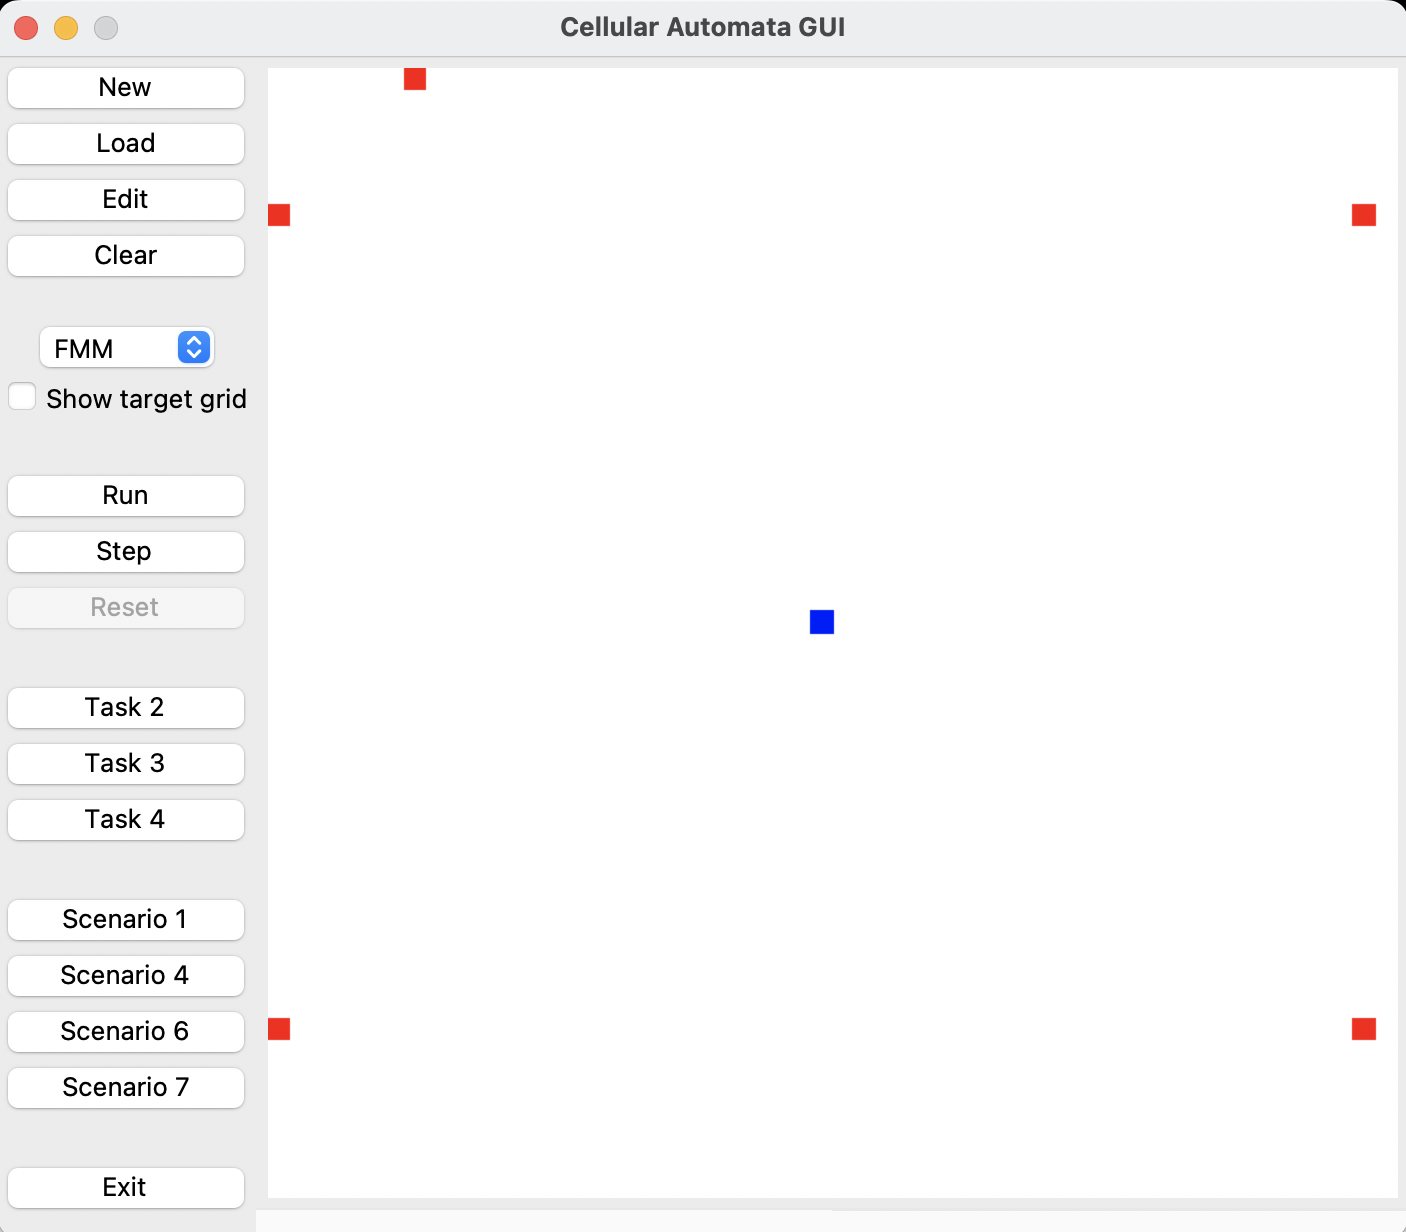
\includegraphics[width=0.3\textwidth]{task3_1}}
  \subfloat[In the middle of the simulation]{
   \label{2a}
    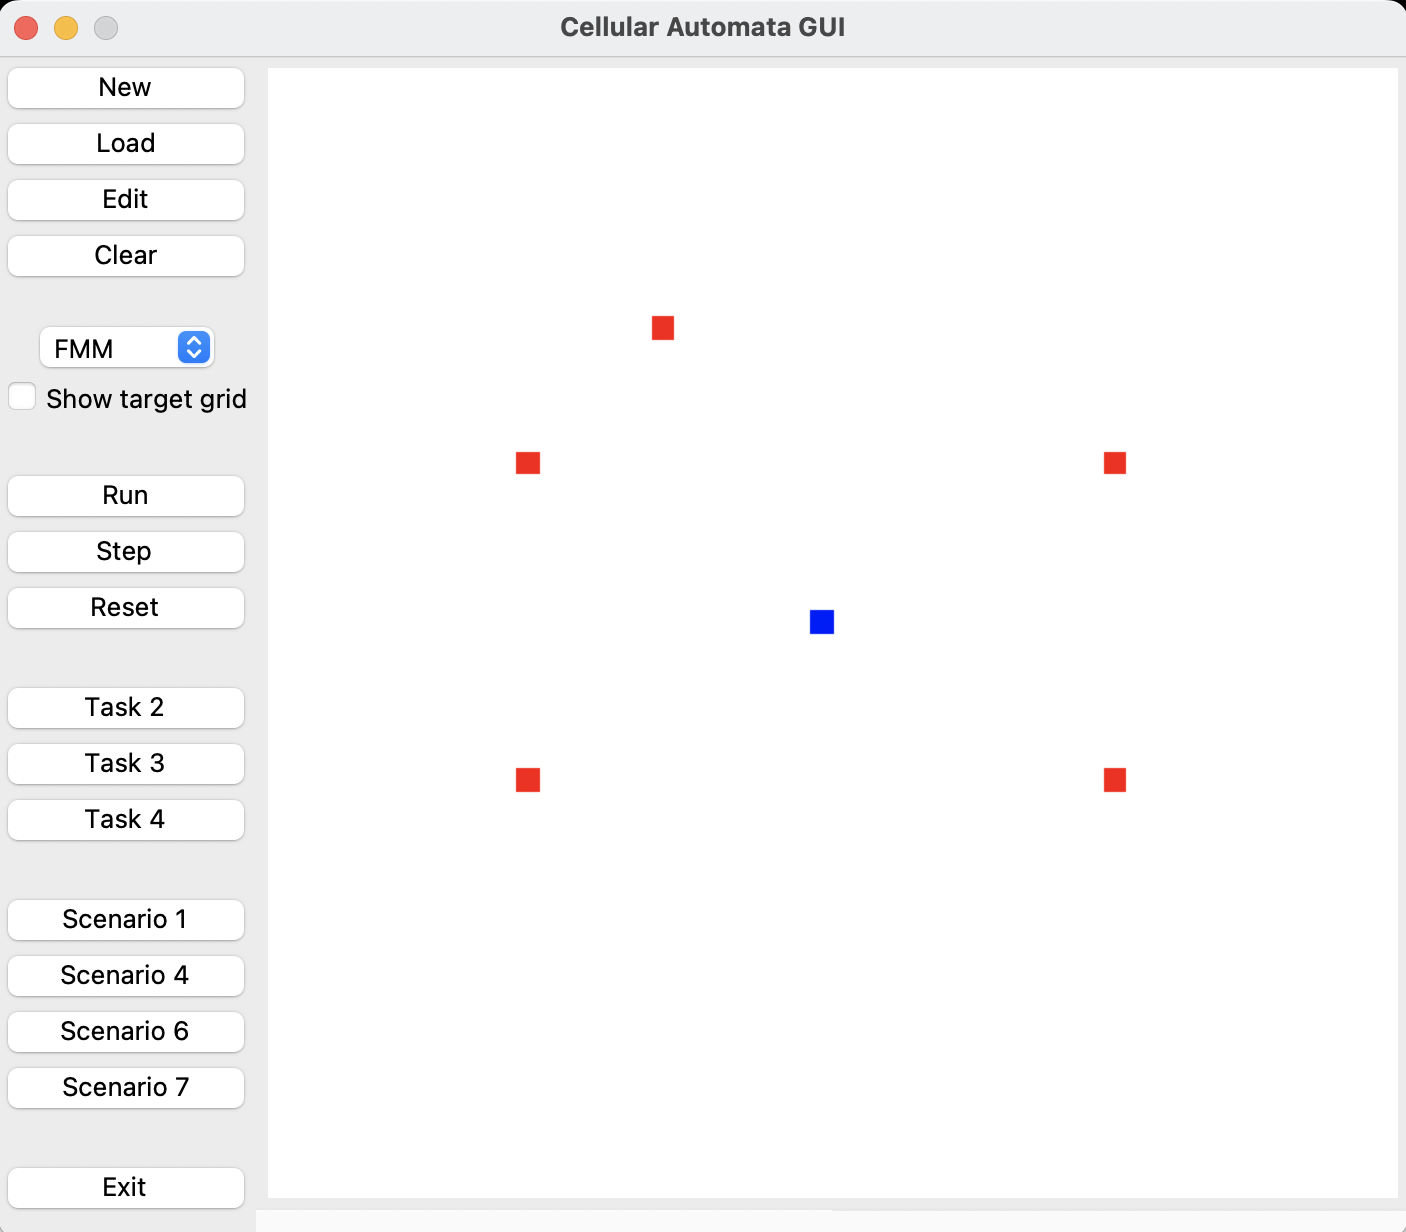
\includegraphics[width=0.3\textwidth]{task3_2}}
  \subfloat[End of the simulation]{
   \label{3a}
    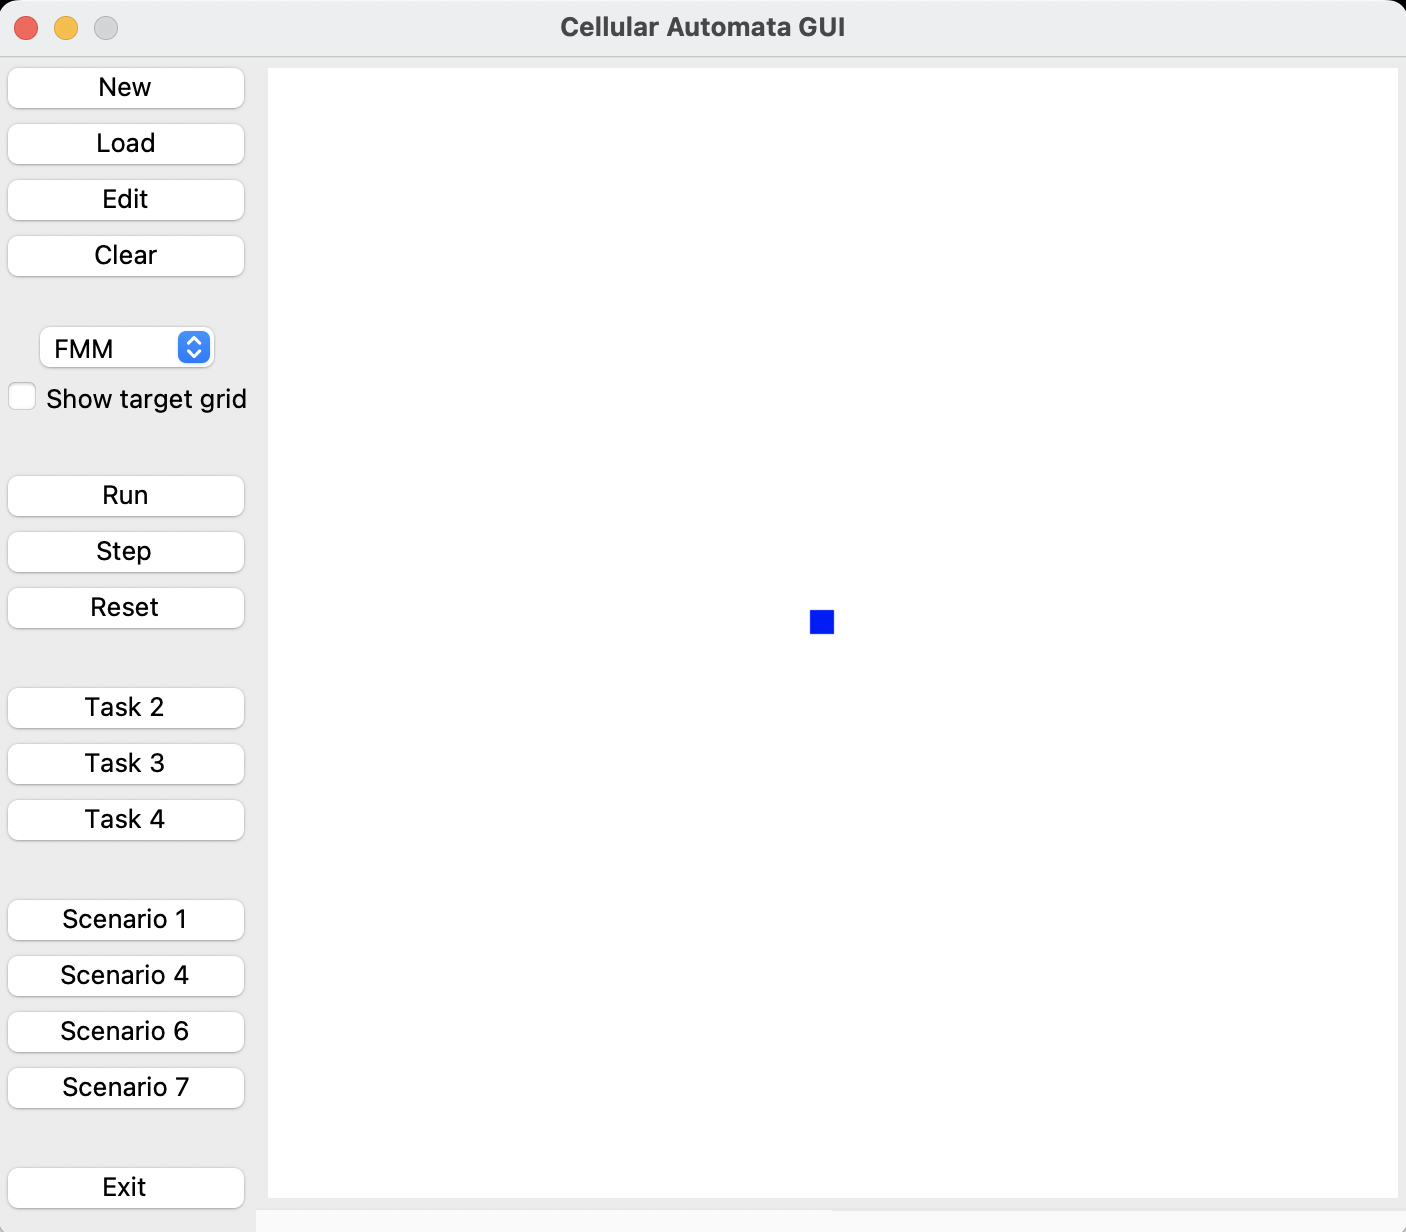
\includegraphics[width=0.3\textwidth]{task3_3}}
 \caption{Screenshoots showing the different stages of the simulation}
 \label{f2}
\end{figure}

\end{task}


\pagebreak

\begin{task}{4, Obstacle avoidance}
Task 4 consists of different implementation of obstacle avoidance functions. To test the performance of these algorithms, we constructed the environment consisting of two different scenarios, the bottleneck and the "chicken test". For both scenarios, 150 pedestrians were distributed randomly and uniformly within the respective areas. 

\begin{figure}[h]
    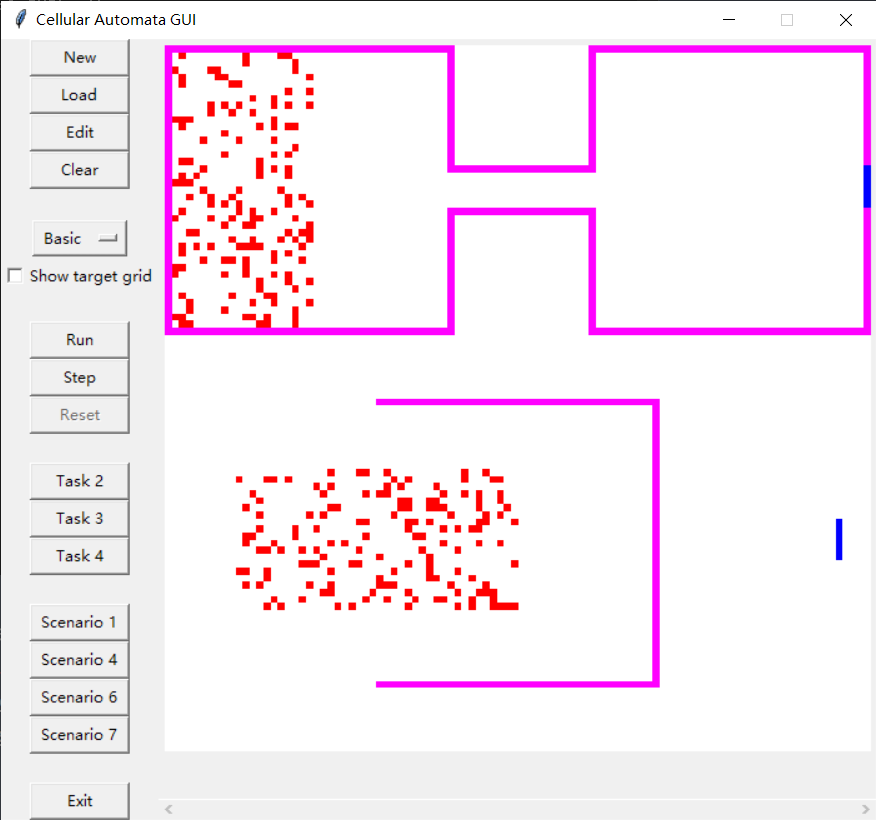
\includegraphics[width=8cm]{task4_1}
    \centering
    \caption{The bottleneck and "chicken test" scenarios}
    \label{fig4_1}
\end{figure}

First, for the rudimentary obstacle avoidance for pedestrians (i.e., without obstacle avoidance algorithms), all pedestrians moves with no a priori knowledge of obstacles, but only considering direction towards the nearest target, thus cannot pass the "chicken test" scenarios successfully. However, they managed to successfully pass the bottleneck scenario, although instead of going straight towards the bottleneck for exiting the first room, they rushed to the right and slowly walk along the wall to the outlet. This is because there is still a descending component of the distance gradient that pointing towards the correct direction at the boundaries around the bottleneck, which is similar to the case in the RiMEA scenario 6 of task 5.

\begin{figure} [!h]
 \centering
  \subfloat[In the middle of the simulation]{
   \label{421}
    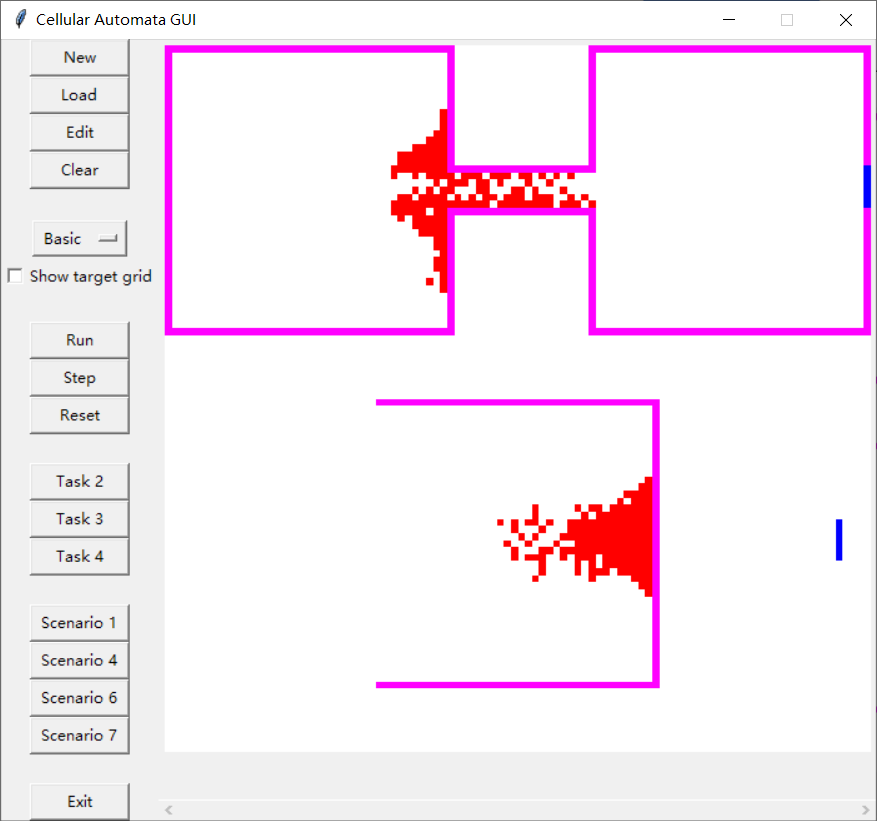
\includegraphics[width=0.3\textwidth]{task4_2_1}}
  \subfloat[Near the end of the simulation]{
   \label{422}
    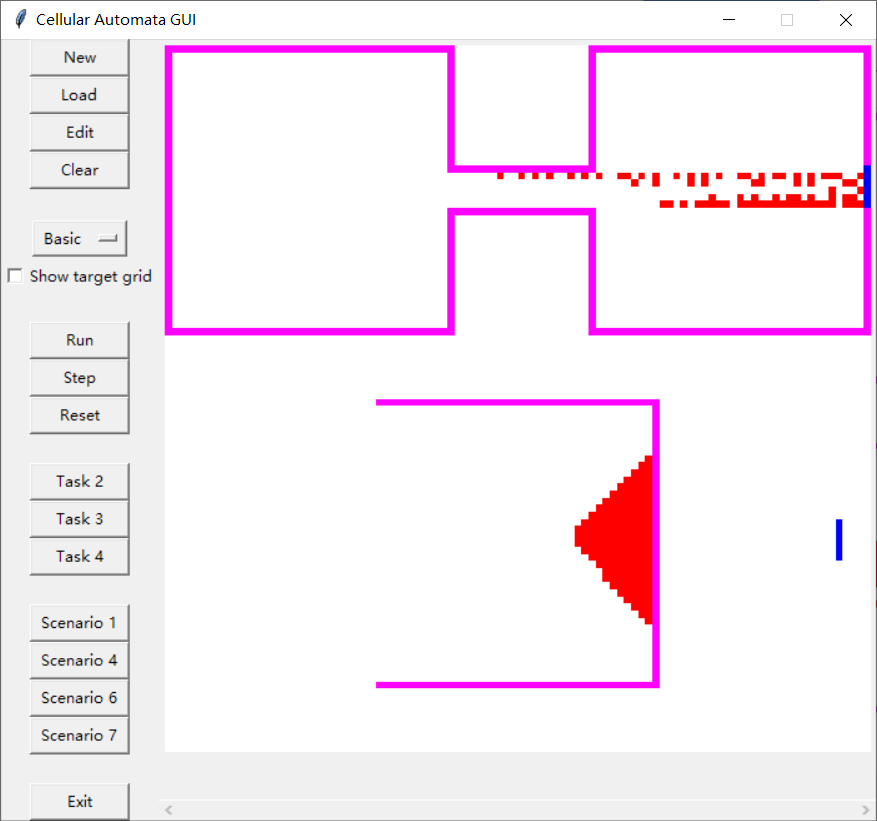
\includegraphics[width=0.3\textwidth]{task4_2_2}}
 \caption{With the basic algorithm, pedestrians failed the "chicken test", but eventually managed to pass the bottleneck scenario}
 \label{f42}
\end{figure}

To solve this problem, we firstly implemented the na\"ive Dijkstra algorithm for flooding cells with distance values from the cells at the target to the entire map. 

\begin{algorithm}[H]
	\caption{Dijkstra Flooding on Distance Map} 
	\label{alg:update_ste}
	\begin{algorithmic}[1]
	    \State closed[] = FALSE
	    \State closed[target cell positions] = TRUE
	    \State distances[] = $\infty$
	    \State distances[target cell positions]
	    \State open positions = get open neighbors(closed positions)
	    \State step counter = 1
		\While {step counter  $<$ step limit AND NOT open positions is empty}
		    \State next open positions = []
			\For {each open position}
			    \State distances[open position] = the neighbors' smallest distance + distance to that neighbor
			    \State closed[open position] = TRUE
			    \State next open positions += (get open neighbors(closed))
			\EndFor
			\State open positions = next open positions
			\State step counter += 1
		\EndWhile
	    \State return distances
	\end{algorithmic} 
\end{algorithm}

Based on such algorithm, the distance grid is now flooding from the target to every reachable cells on the map, and the pedestrians can reach the targets in both scenarios. Result of the experiment is shown in Figure \ref{f43} on the following page.

\begin{figure} [!h]
 \centering
  \subfloat[At the beginning of the simulation]{
   \label{431}
    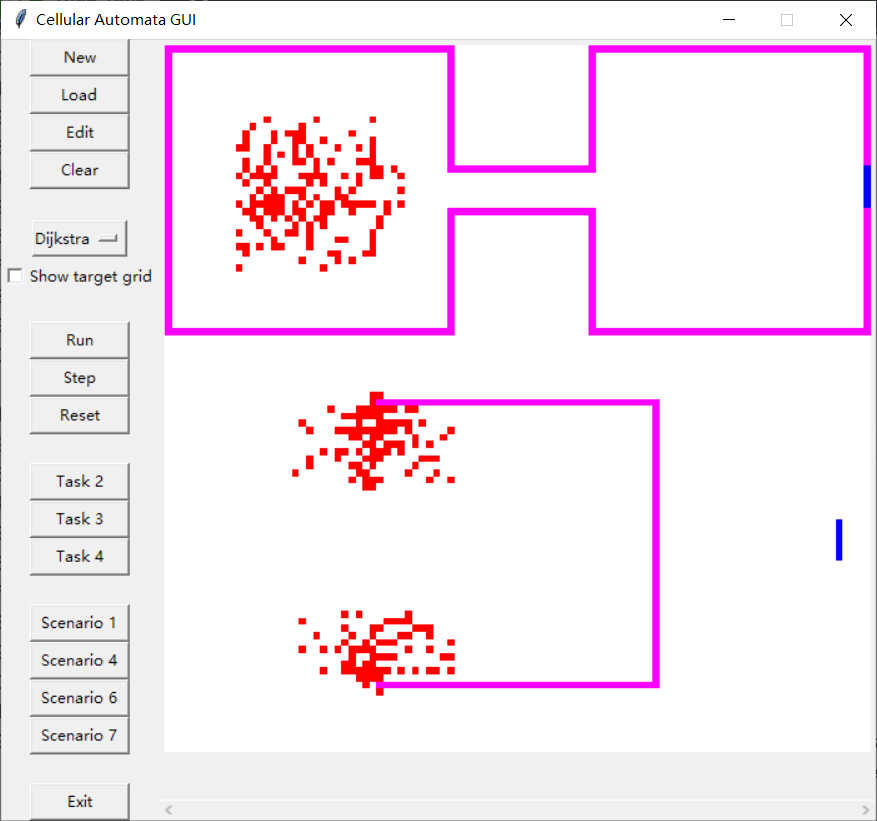
\includegraphics[width=0.3\textwidth]{task4_3_1}}
  \subfloat[In the middle of the simulation]{
   \label{432}
    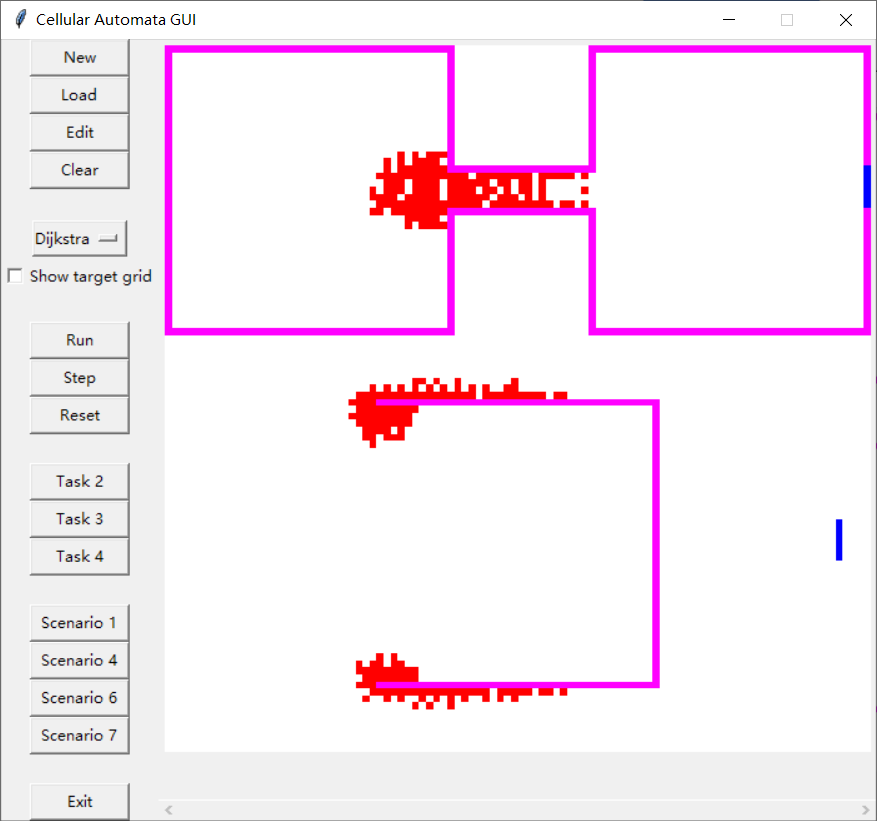
\includegraphics[width=0.3\textwidth]{task4_3_2}}
  \subfloat[Near the end of the simulation]{
   \label{433}
    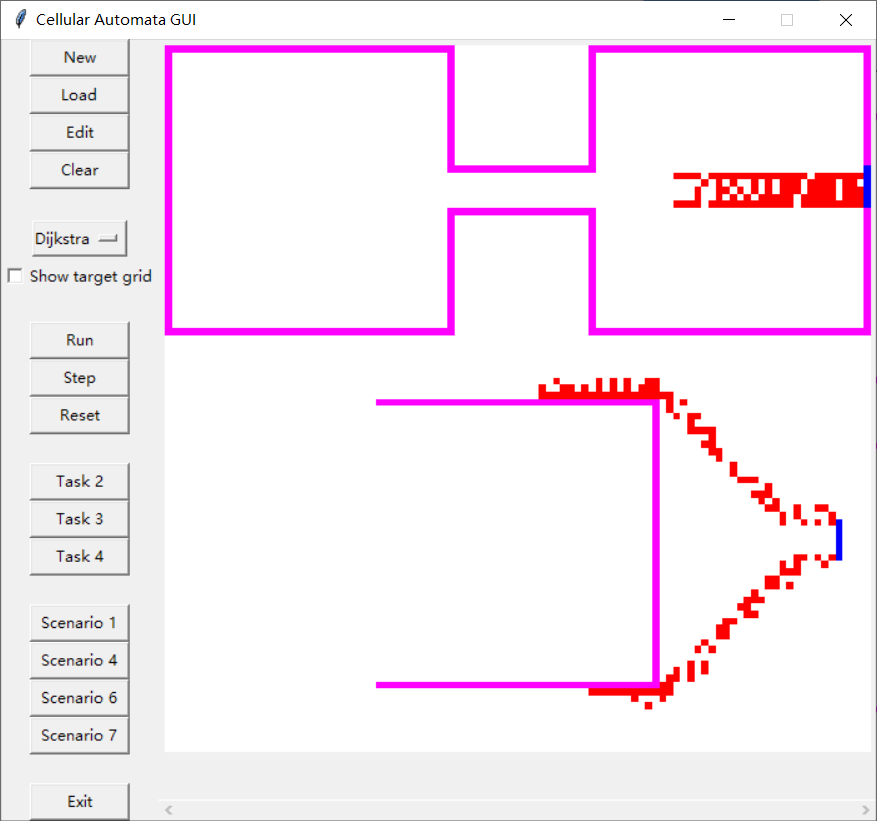
\includegraphics[width=0.3\textwidth]{task4_3_3}}
 \caption{With the Dijkstra flooding algorithm, pedestrians gained the ability to pass all obstacles and can pass both scenarios now}
 \label{f43}
\end{figure}

In order to have a more accurate computation of the distance field, we also implemented the Fast Marching Method by Sethian, using a third-party function provided in the library \textbf{scikit-fmm}. The process of flooding computation and the behavior of pedestrians are similar in both Dijkstra and FMM algorithms, for which and due to space constraints we are not presenting the pseudo-code and images of pedestrians again. 

The following figure shows the different result of the distance field computed by the basic, Dijkstra and FMM algorithms (Figure \ref{f44}). From which we can see that the basic algorithm failed to take any obstacles into consideration, the Dijkstra one shows a clear eight-maned star pattern, which was generated because each cell's distance is calculated on the basis of the eight neighbors' distances, rather than a real representation of distance towards the target. And the result from FMM algorithm has shown an accurate, smooth distance field, with values representing the true distance to the nearest target, which has the best performance among these three algorithms.

\begin{figure} [H]
 \centering
  \subfloat[The Basic Algorithm]{
   \label{431}
    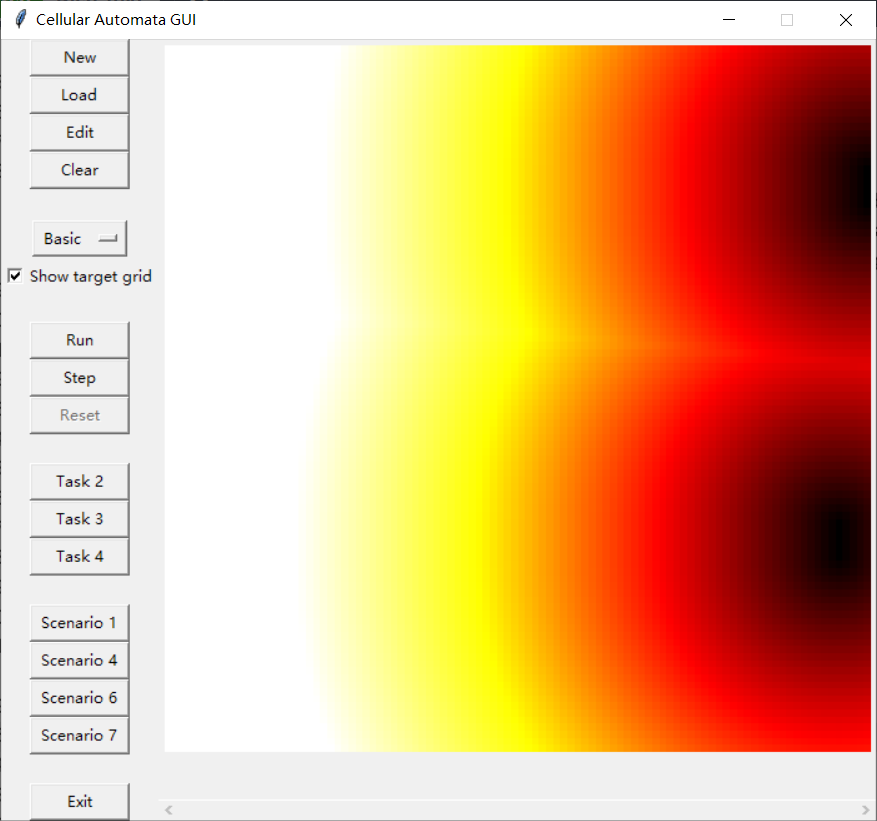
\includegraphics[width=0.3\textwidth]{task4_4_1}}
  \subfloat[The Dijkstra Flooding Algorithm]{
   \label{432}
    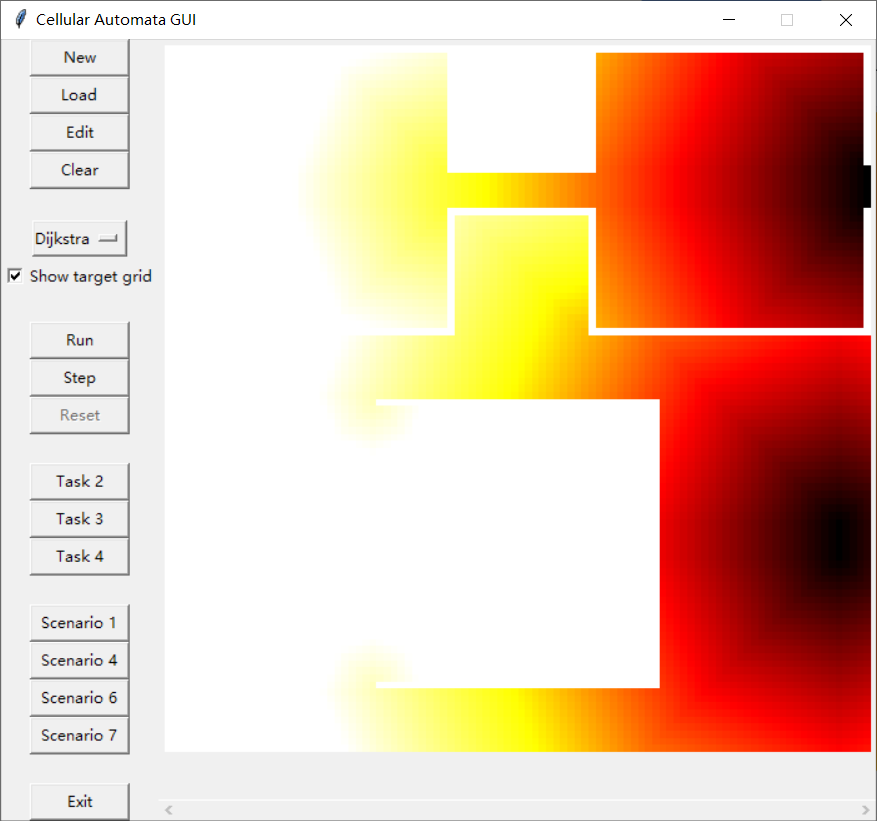
\includegraphics[width=0.3\textwidth]{task4_4_2}}
  \subfloat[The Fast Marching Method]{
   \label{433}
    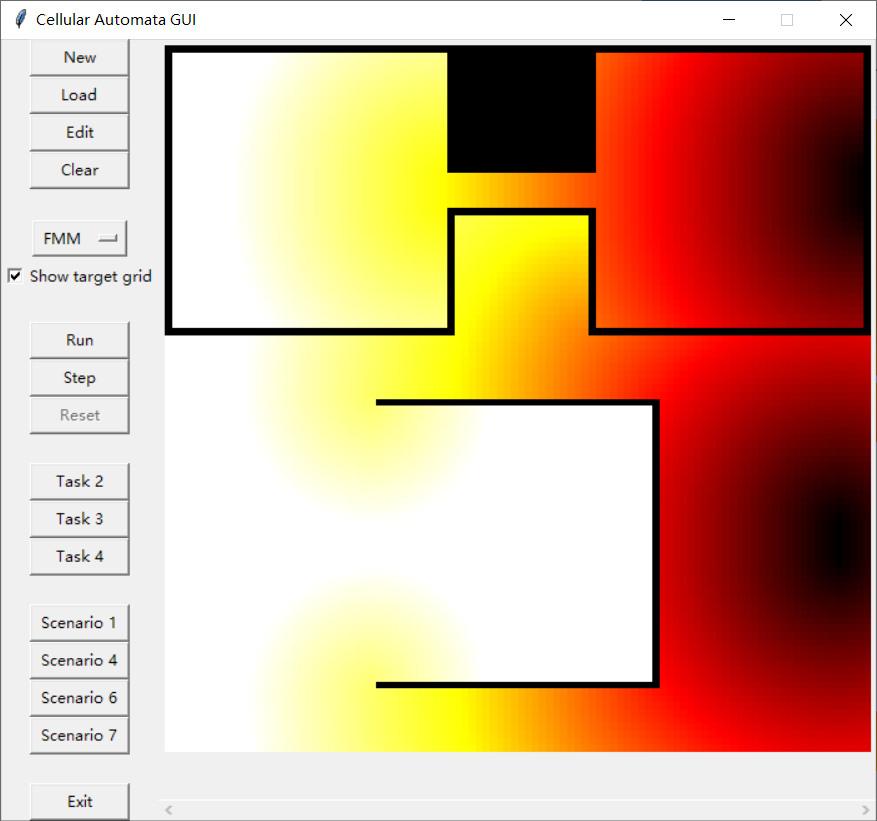
\includegraphics[width=0.3\textwidth]{task4_4_3}}
 \caption{Result of the distance field computed by different algorithms}
 \label{f44}
\end{figure}

\end{task}

\pagebreak 

\begin{task}{5, Tests}

\noindent{\textbf{TEST1: RiMEA scenario 1 (straight line)}}

The RiMEA scenario 1 consists in a single pedestrian with 40 cm body dimension located in the beginning of a 2m wide and 40m long corridor (Figure \ref{fig10}). This scenario tries to show that a pedestrian with a defined walking speed will cover the distance in the corresponding time period.

For this scenario, it has been consider that a cell has 40cm x 40cm dimensions. So that, the pedestrian of 40cm body dimension is located only in one cell. The corridor then will be 100 cells (100 x 40cm = 40m) away from the pedestrian and as the pedestrian has a walking speed of 1.3m/step = 3.25 cells/step, the pedestrian will have to reach the target after 31 steps (100/3.25 = 30.76).

\begin{figure}[!h]
    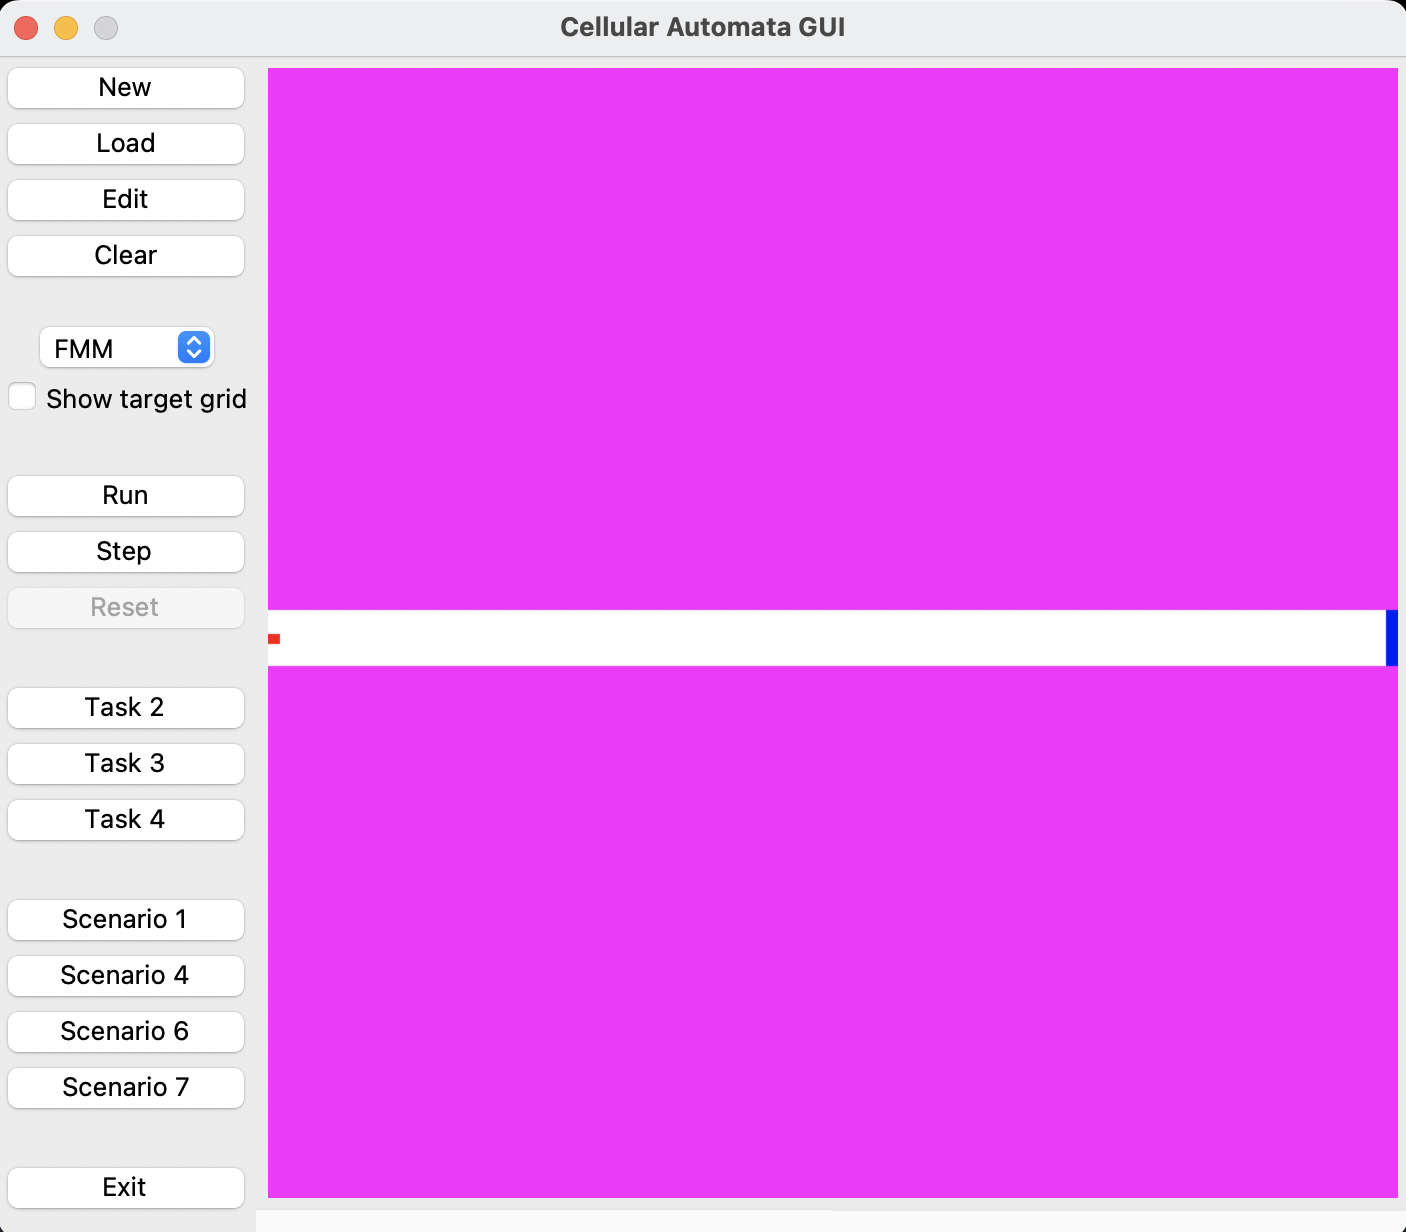
\includegraphics[width=6cm]{test1_1}
    \centering
    \caption{Initial setup of the scenario}
    \label{fig10}
\end{figure}

In fact, after doing the simulation the pedestrian has reached the target after 31 steps.



\noindent{\textbf{TEST2: RiMEA scenario 4 (fundamental diagram: density vs. velocity or density vs. flow)}}

The RiMEA scenario 4 describes a corridor (1000 m long, 10 m wide) to be filled with different densities 
of persons with an equal as possible free walking 
speed (for example 1.2 – 1.4m/s): 0.5 P/m², 1 P/m², 
2 P/m², 3 P/m², 4 P/m², 5 P/m² and 6 P/m². Considering that the original corridor is too long to implement and display the results efficiently, we hereby only select the 200m part in the middle of the corridor to test our algorithms. Based on the implemented function to fill in pedestrians according to given densities, we further provided GUI for choosing the aforementioned densities, and test the corresponding behaviors within the corridor. 

\begin{figure} [!h]
 \centering
  \subfloat[Density = 0.5 P/m²]{
   \label{den2}
    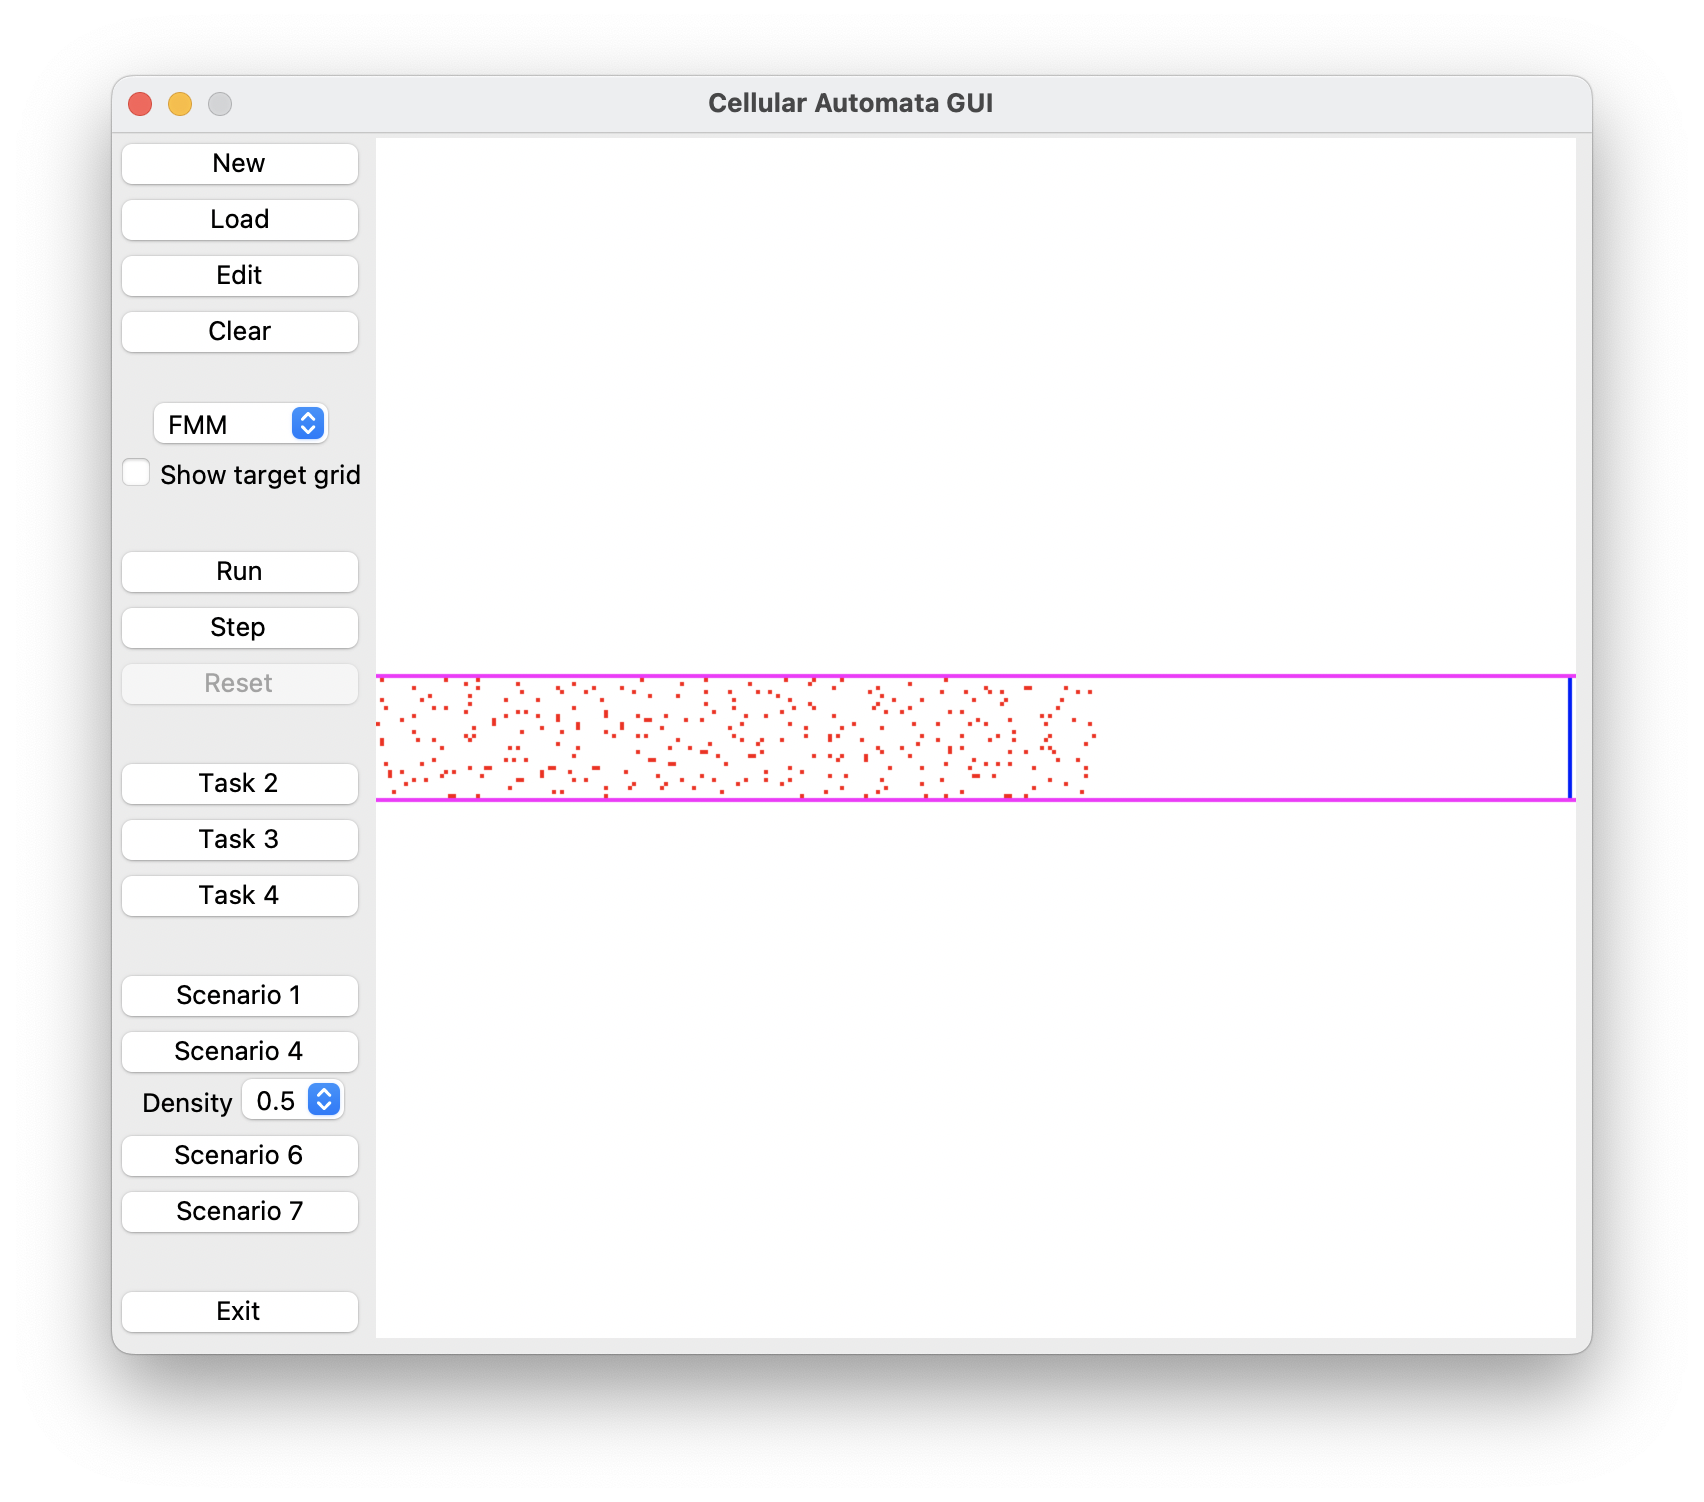
\includegraphics[width=0.5\textwidth]{den0.5}}
  \subfloat[Density = 4 P/m²]{
   \label{den4}
    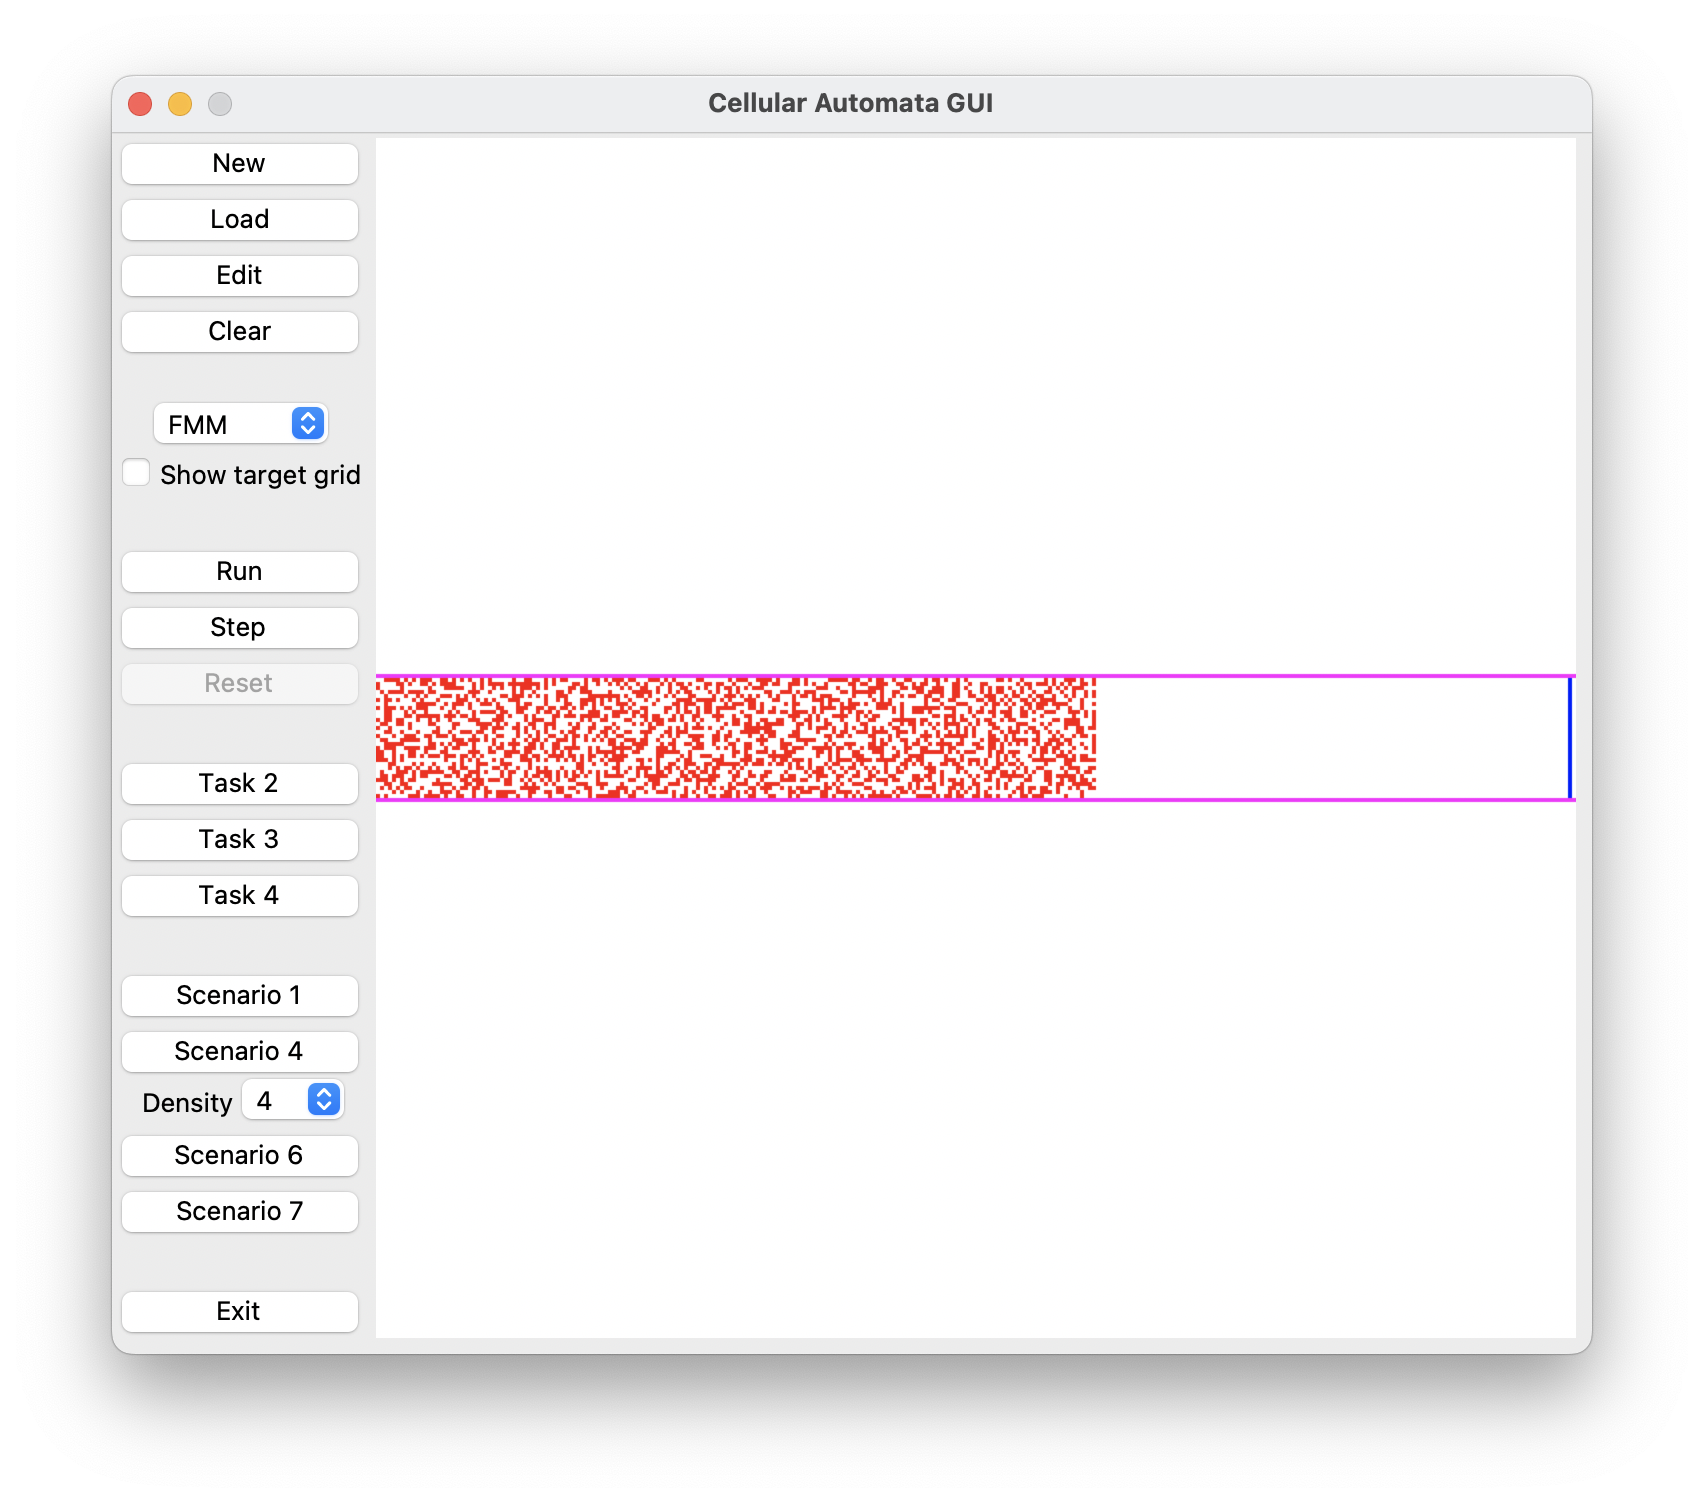
\includegraphics[width=0.5\textwidth]{den4}}
 \caption{GUI and changed environment for different densities}
 \label{den}
\end{figure}

For the measuring points in the test scenarios, we transformed the original calculation of flow = speed $\times$ density into the number of pedestrians getting across a unit length of border into the measuring area within a unit time unit, i.e., the number of pedestrians passing the left border (for all pedestrians can only move towards right) in each second, divided by the length of the left border. This is based on the calculation that $(m/s) \times (P/m^2) = P/(s\times m)$.

We implemented the gathering information of pedestrians passing borders within the process of updating each pedestrians' positions. For each time a pedestrian's position is updated, it checks for each measuring points whether the pedestrian is the case, that the previous position is outside border (beyond left boundary), and the new position is within the measuring area. If so, then the current time is added into the dictionary containing all measuring points as keys and a list of time that all  pedestrians counted passed through the boundary as values. After all pedestrians reached the destination, the dictionary is exported for aggregation of useful information and eventually calculating the flow. 

Here we show the result of flow over time on all 3 measuring points for 3 different densities of pedestrians: 6P/m², 4P/m² and 2P/m², in the Figure \ref{s42}. From which we can see that the system managed to capture the characteristic of "overcrowding", that is the non-linear relation between increase in density, flow and total time used for all pedestrians to reach the target.



\begin{figure}[H]
    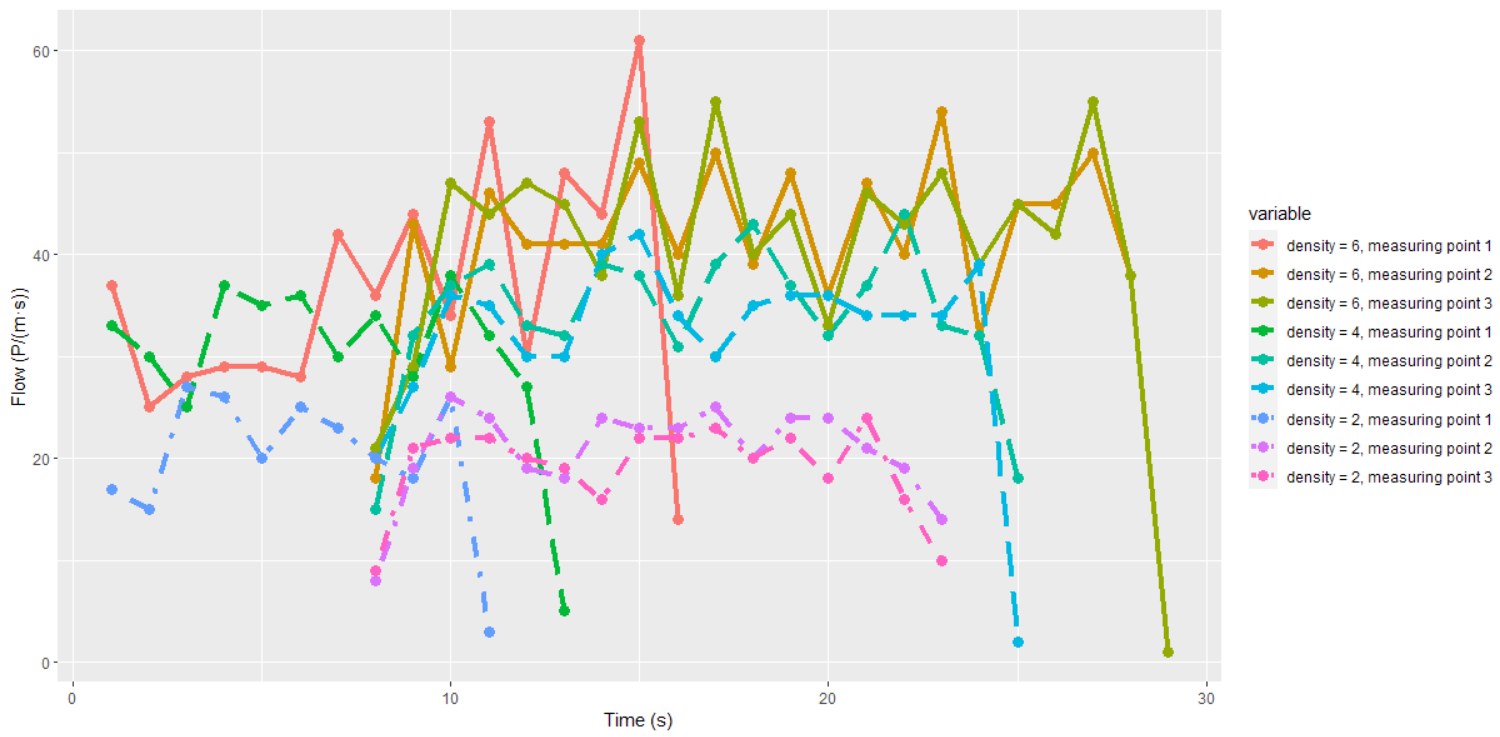
\includegraphics[width=14cm]{scenario_4_2}
    \centering
    \caption{Flow over time for different densities, counted at 3 measuring points}
    \label{s42}
\end{figure}

As we can see, the increase of density from 2 to 4 has caused more increase in flow, and also less increase in total evacuation time, than the one of density from 4 to 6. It also seems that the total amount of area beneath the line of flow over time stays linear with the density, and the more dense pedestrians has gathered from the beginning, the less efficient they are in moving towards the target, and the longer time it takes for all of them to reach the target. Reasonable result like this indeed proved that our simulation is able to successfully display basic features of crowd dynamics.


\noindent{\textbf{TEST3: RiMEA scenario 6 (movement around a corner)}}

The RiMEA scenario 6 describes a group of 20 pedestrians moving towards a corner which turns to the left (Figure \ref{1b}) will successfully go around it without passing through walls. The objective of this scenario is to show that the pedestrians in the simulation can avoid the obstacles.

\begin{figure} [H]
 \centering
  \subfloat[Initial setup of the scenario]{
   \label{1b}
    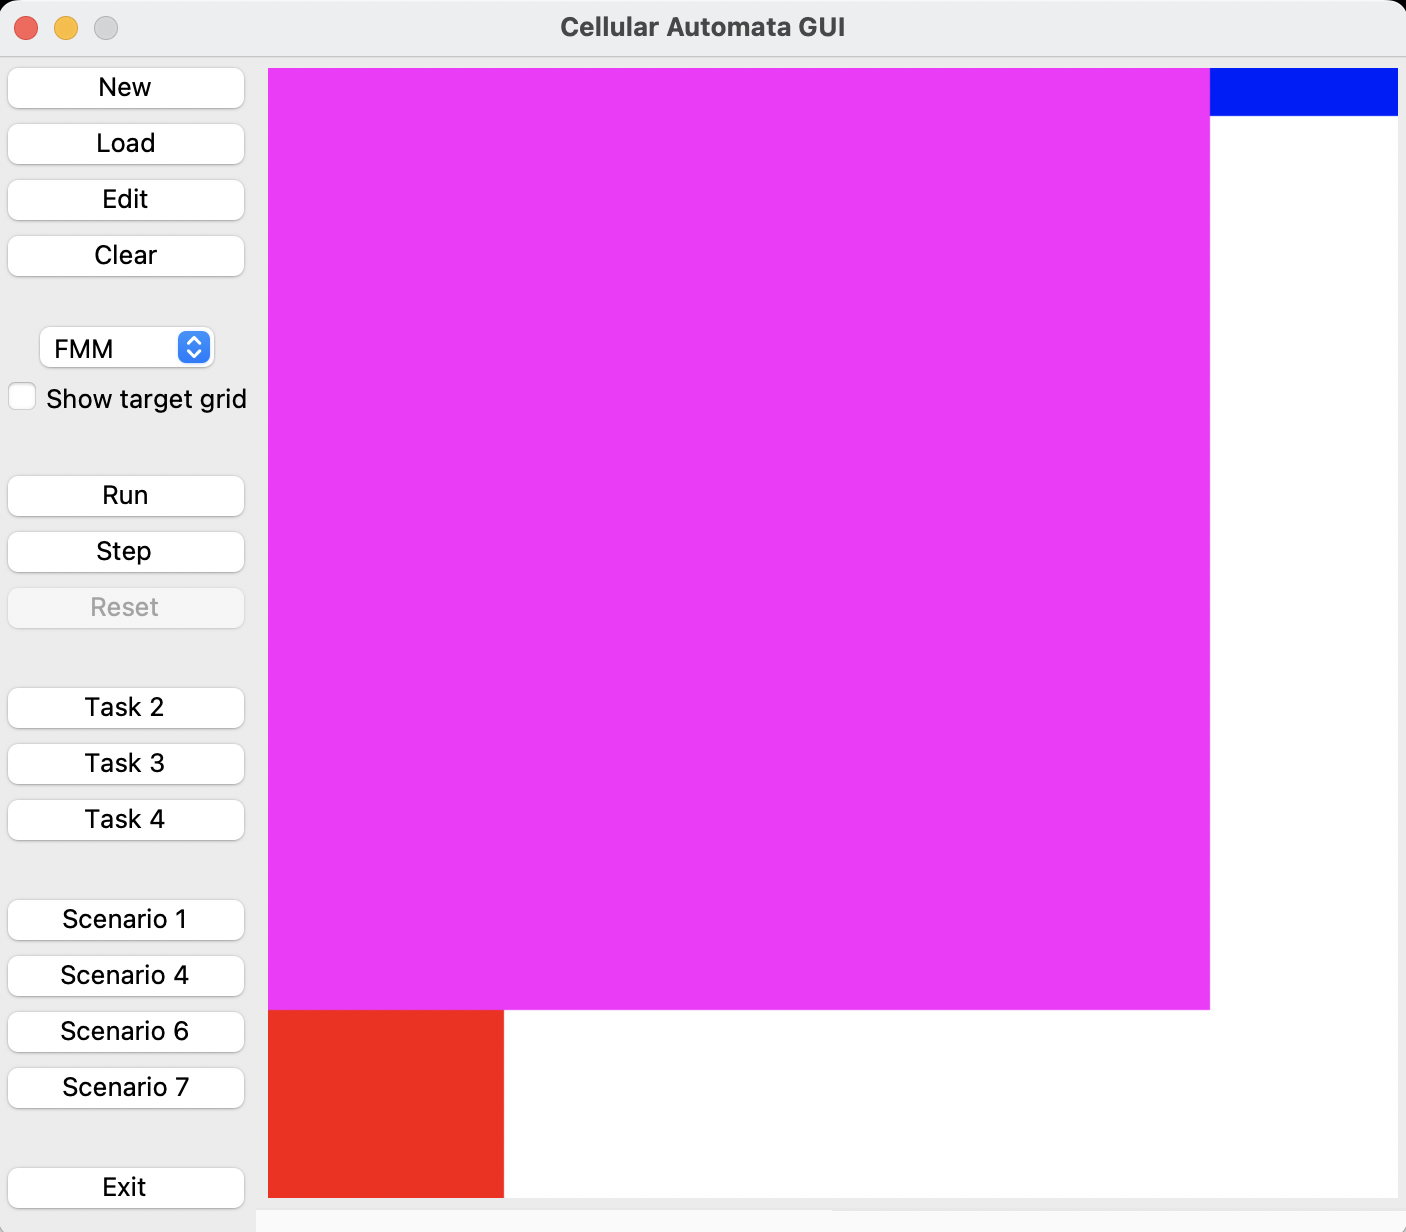
\includegraphics[width=0.3\textwidth]{test3_1}}
  \subfloat[In the middle of the simulation]{
   \label{2b}
    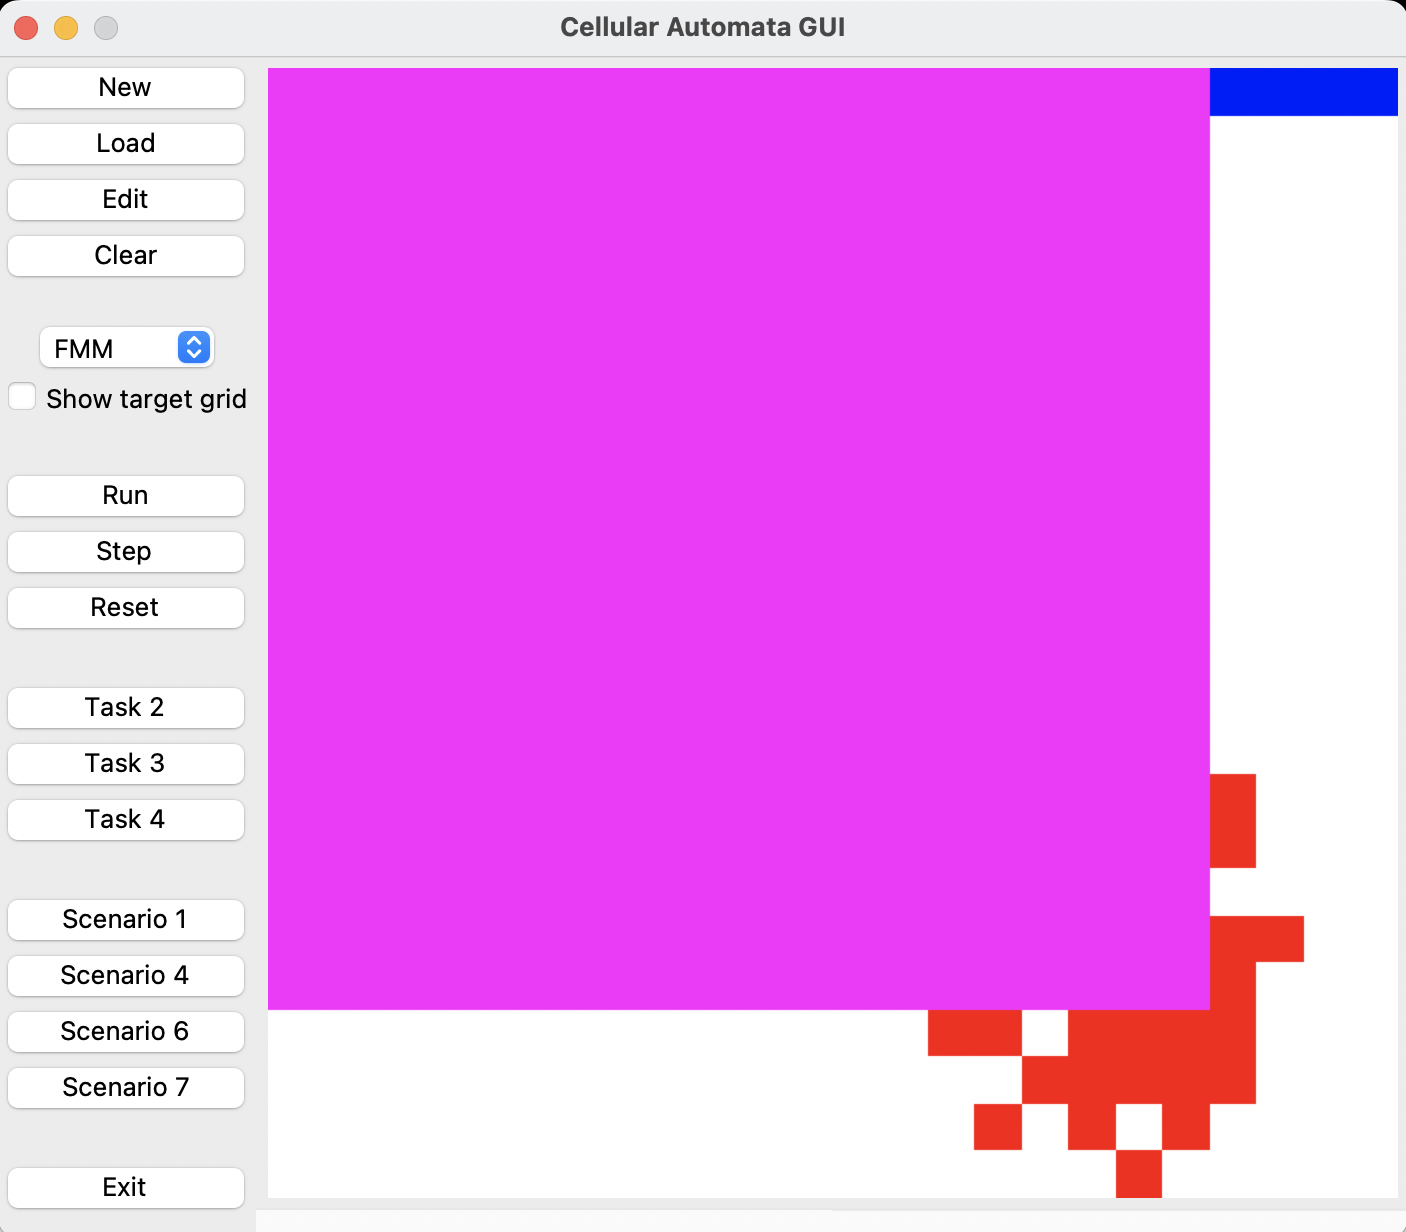
\includegraphics[width=0.3\textwidth]{test3_2}}
  \subfloat[End of the simulation]{
   \label{3b}
    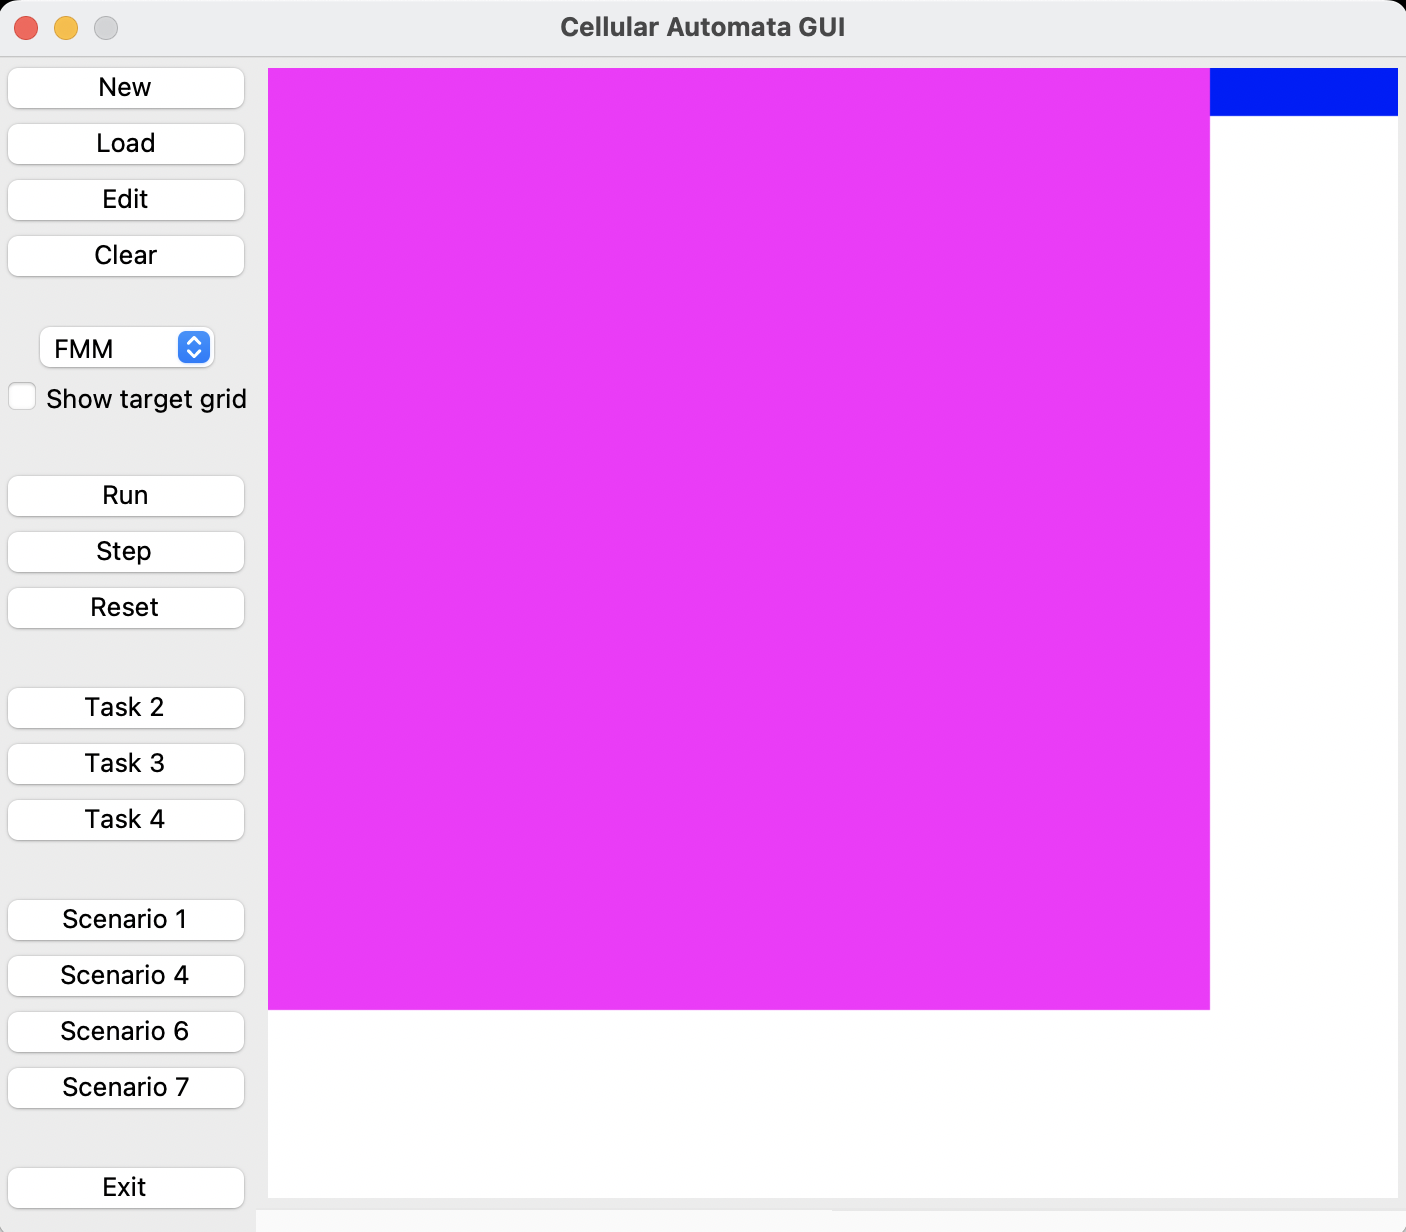
\includegraphics[width=0.3\textwidth]{test3_3}}
 \caption{Screenshoots showing the different stages of the simulation}
 \label{f3}
\end{figure}

In fact, the pedestrians can avoid the wall (Figure \ref{2b}) and reach the targets (Figure \ref{3b}).

\noindent{\textbf{TEST4: RiMEA scenario 7 (demographic parameters)}}

The RiMEA scenario 7 describes a group of 50 pedestrians aged between 18 and 80, with walking speeds distributed in accordance with Figure \ref{fig_sc7}. The aim of this scenario is to show that the distribution of walking speeds in the simulation is consistent with the distribution in the table.

\begin{figure}[H]
    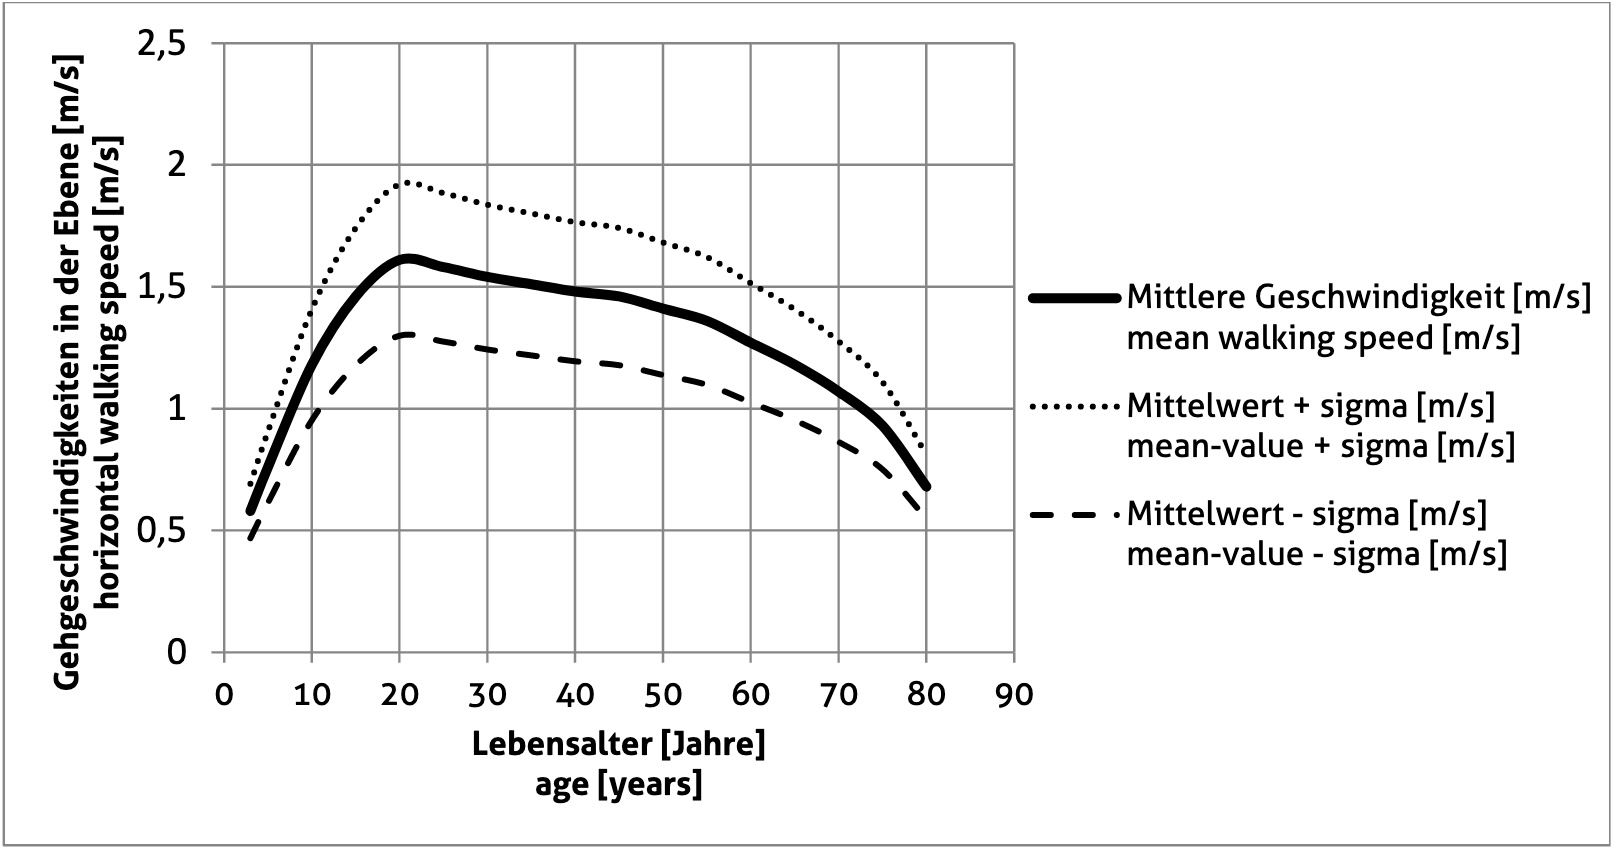
\includegraphics[width=12cm]{images/walking_speed.jpg}
    \centering
    \caption{Walking speed in the plane as a function of age based on Weidmann \cite{weidmann}}
    \label{fig_sc7}
\end{figure}

For this task, the main feature implemented was the assignment of the walking speeds to pedestrians depending on their ages. By taking a look at the Figure \ref{fig_sc7}, it can be seen that the distribution does not follow any pattern, so the implementation had to be done in an approximate way. Therefore, for every different age interval, a mean walking speed and a standard deviation has been assigned (another option would have been taking every single age and attributing it its corresponding walking speed and sigma parameter, but defining age intervals should be enough if accuracy is not the main objective). By doing so, the walking speeds can be assigned with a normal distribution so that with a large enough number of pedestrians or different executions, on average, the results would be as similar as possible to the figure. The implementation of this feature is shown in Listing \ref{assign_speeds}
\vspace{30mm}
\begin{lstlisting}[language=Python, caption=Normal distribution of walking speeds depending on different age intervals, xleftmargin=.17\textwidth, label={assign_speeds}]
def assign_speeds(self):
    for pedestrian in self.pedestrians:
        age = pedestrian.age
        if age < 20:
            mean_speed = 1.5
            std = 0.3
        elif age >= 20 and age < 30:
            mean_speed = 1.6
            std = 0.25
        elif age >= 30 and age < 40:
            mean_speed = 1.5
            std = 0.25
        elif age >= 40 and age < 50:
            mean_speed = 1.4
            std = 0.25
        elif age >= 50 and age < 60:
            mean_speed = 1.3
            std = 0.2
        elif age >= 60 and age < 70:
            mean_speed = 1.1
            std = 0.1
        else:
            mean_speed = 0.9
            std = 0.1

    pedestrian._desired_speed = np.random.normal(mean_speed, std)
\end{lstlisting}

The scenario has dimensions 50x50, with 50 pedestrians placed in the first column and 50 targets placed in the last column, as shown in Figure \ref{scenario_7}. As it can be observed in Figures \ref{scenario_7a} and \ref{scenario_7b}, the pedestrians are moving in different walking speeds as expected, but it must verified that the real walking speed and the assigned walking speed of each pedestrian is roughly the same. Since the measurement units are metres per second, the Euclidean distance unit has been considered as metres and each tick as a second. Therefore, the real speed has been calculated dividing the distance walked by the time spent until reaching the target.


\begin{figure} [H]
 \centering
  \subfloat[Initial setup of the scenario]{
   \label{scenario_7}
    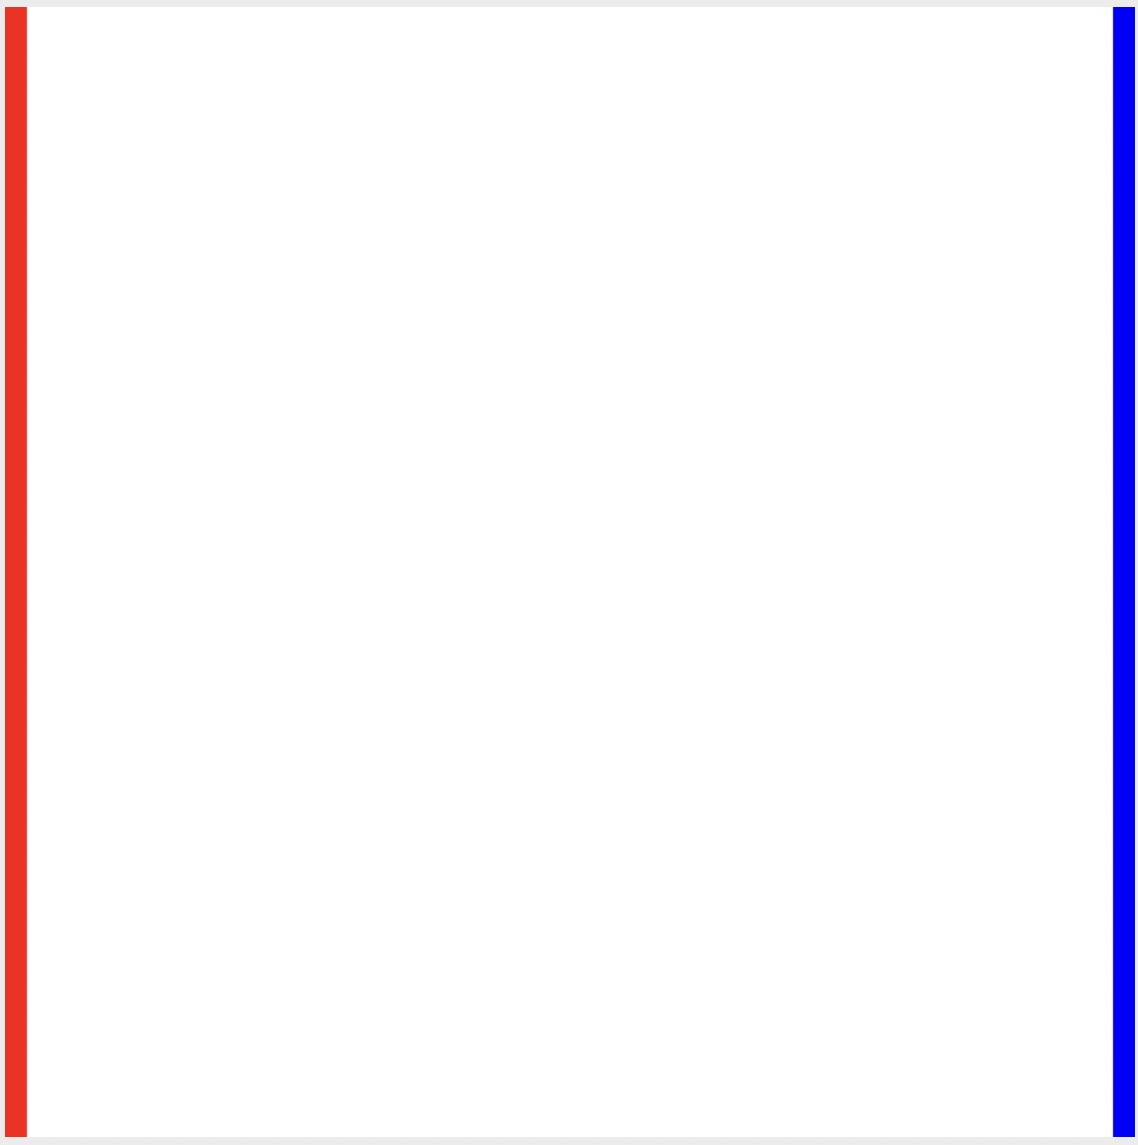
\includegraphics[width=0.3\textwidth]{images/scenario_7.jpg}}
  \subfloat[Start of the simulation]{
   \label{scenario_7a}
    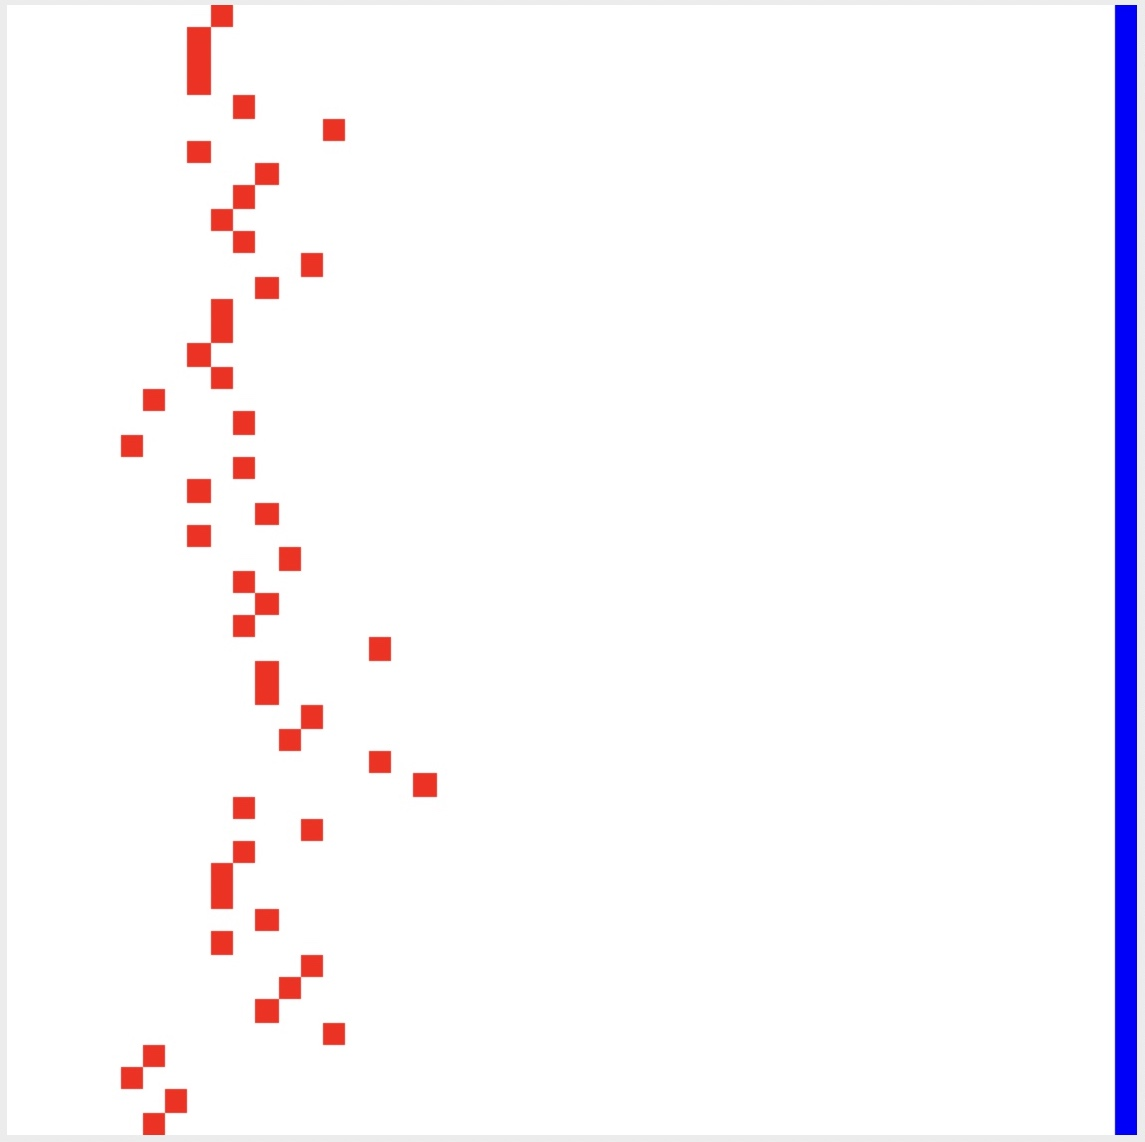
\includegraphics[width=0.3\textwidth]{images/scenario_7a.jpg}}
  \subfloat[Middle of the simulation]{
   \label{scenario_7b}
    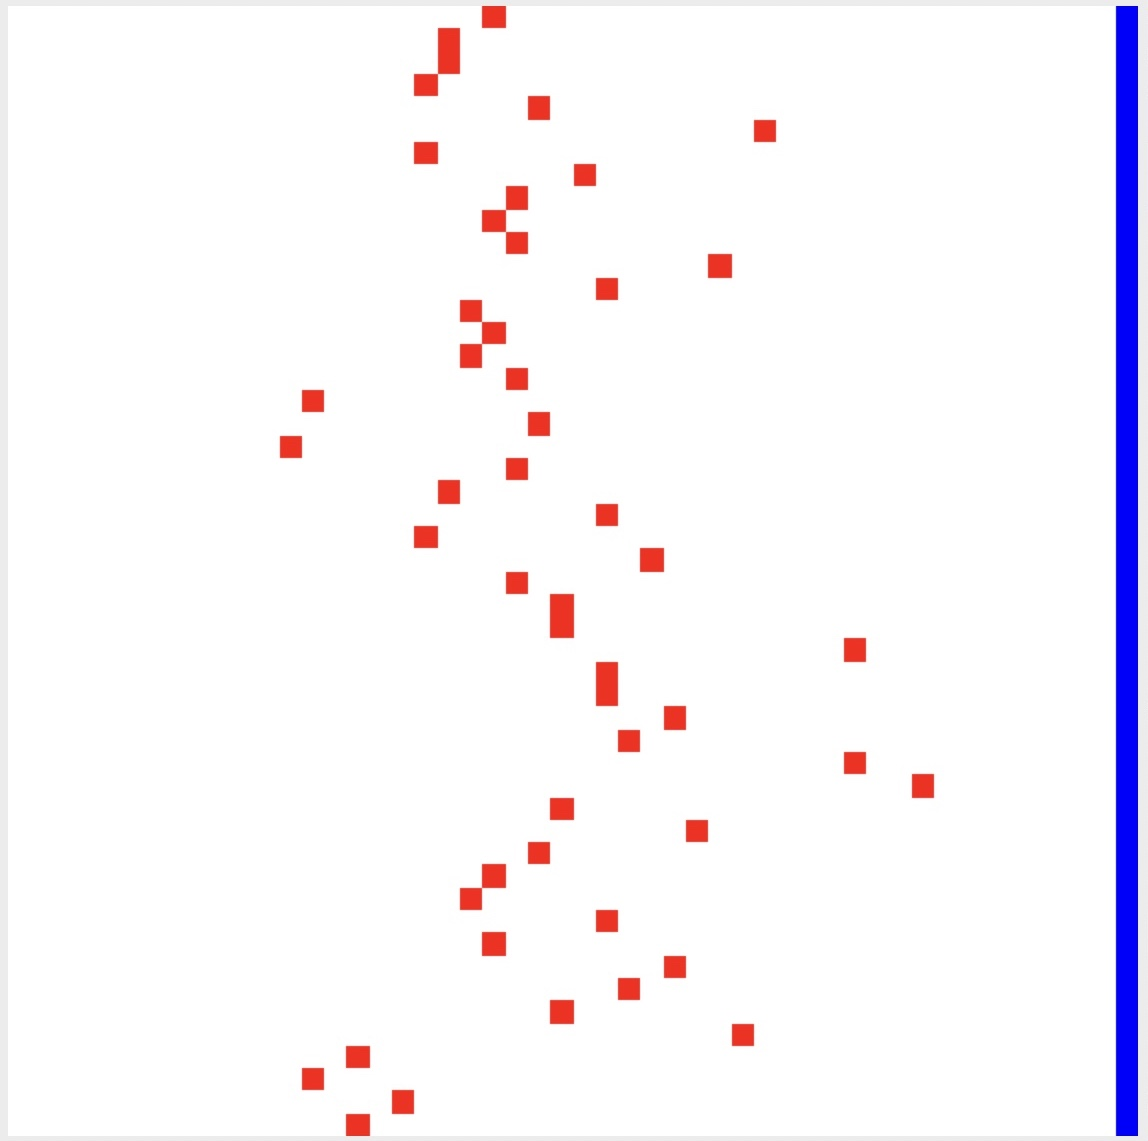
\includegraphics[width=0.3\textwidth]{images/scenario_7b.jpg}}
 \caption{Different stages of the simulation of the scenario 7}
 \label{f3}
\end{figure}

Now, moving on to the results of the simulation, by looking at the Table \ref{pedestrian_recordings}, it can be noticed that there is not much of a difference between the expected speed and the real speed, which means that the implementation for the walking speed is quite accurate. As for the relation between the walking speed and the age of the pedestrians, the experiment done consisted in executing multiple simulations (with randomized ages in each execution) and saving the results, in order to obtain a plot similar to the Figure \ref{fig_sc7}. This statistical test is appropriate since, as it was said before, with the defined normal distribution, the results obtained over a large number of observations should make a good representation of the plot to be recreated. By comparing the obtained scatter plot displayed in Figure \ref{plot500} and the original plot, it can be noticed that there are similarities in the tendency of the mean walking speed as well as in its deviation. Therefore, it has been concluded that both the experiment and the simulation were successful. 

\begin{figure} [H]
 \centering
  \subfloat[Scatter plot with 50 observations]{
   \label{plot50}
    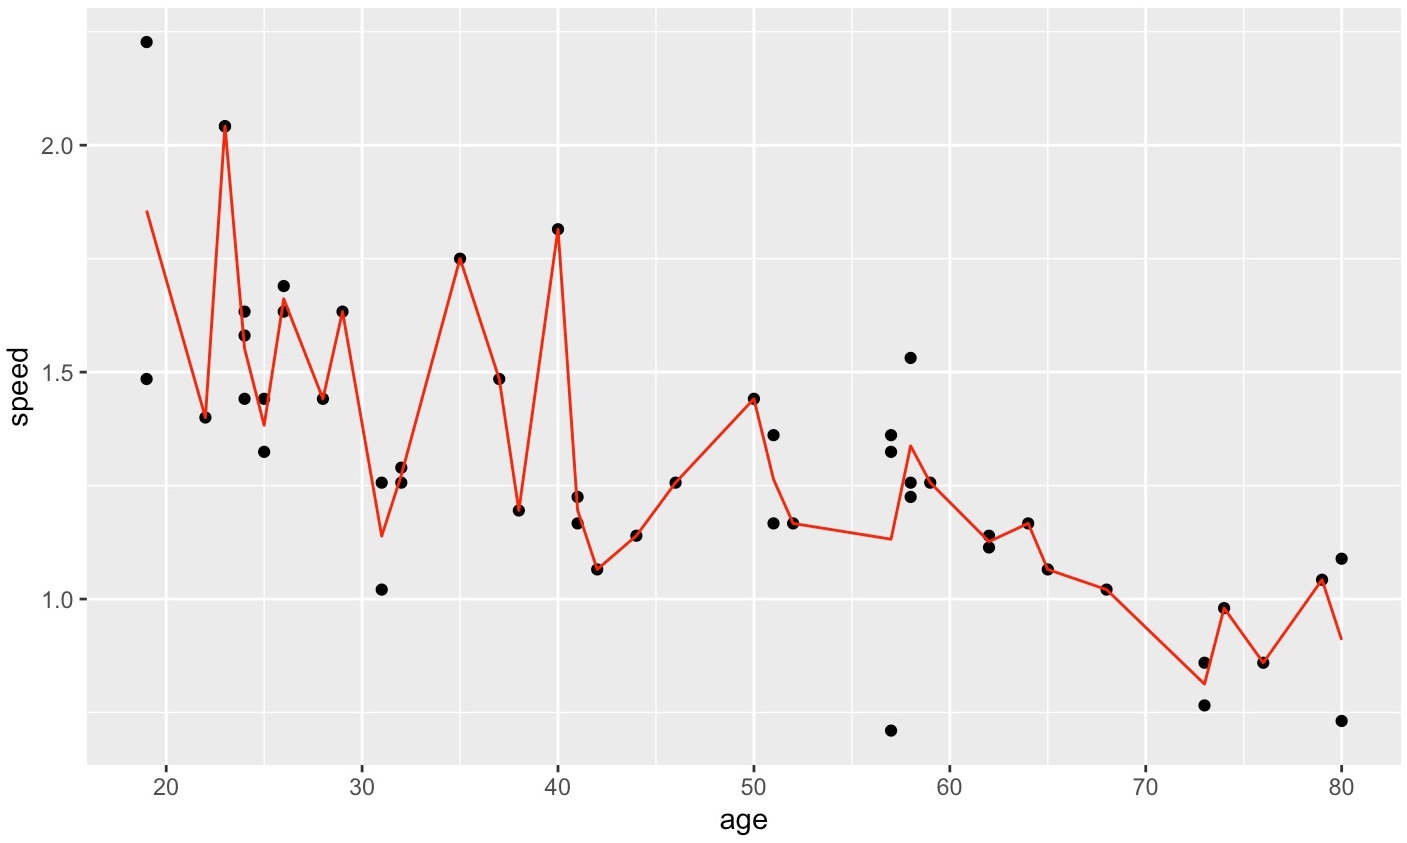
\includegraphics[width=0.5\textwidth]{images/plot50.jpg}}
  \subfloat[Scatter plot with 500 observations]{
   \label{plot500}
    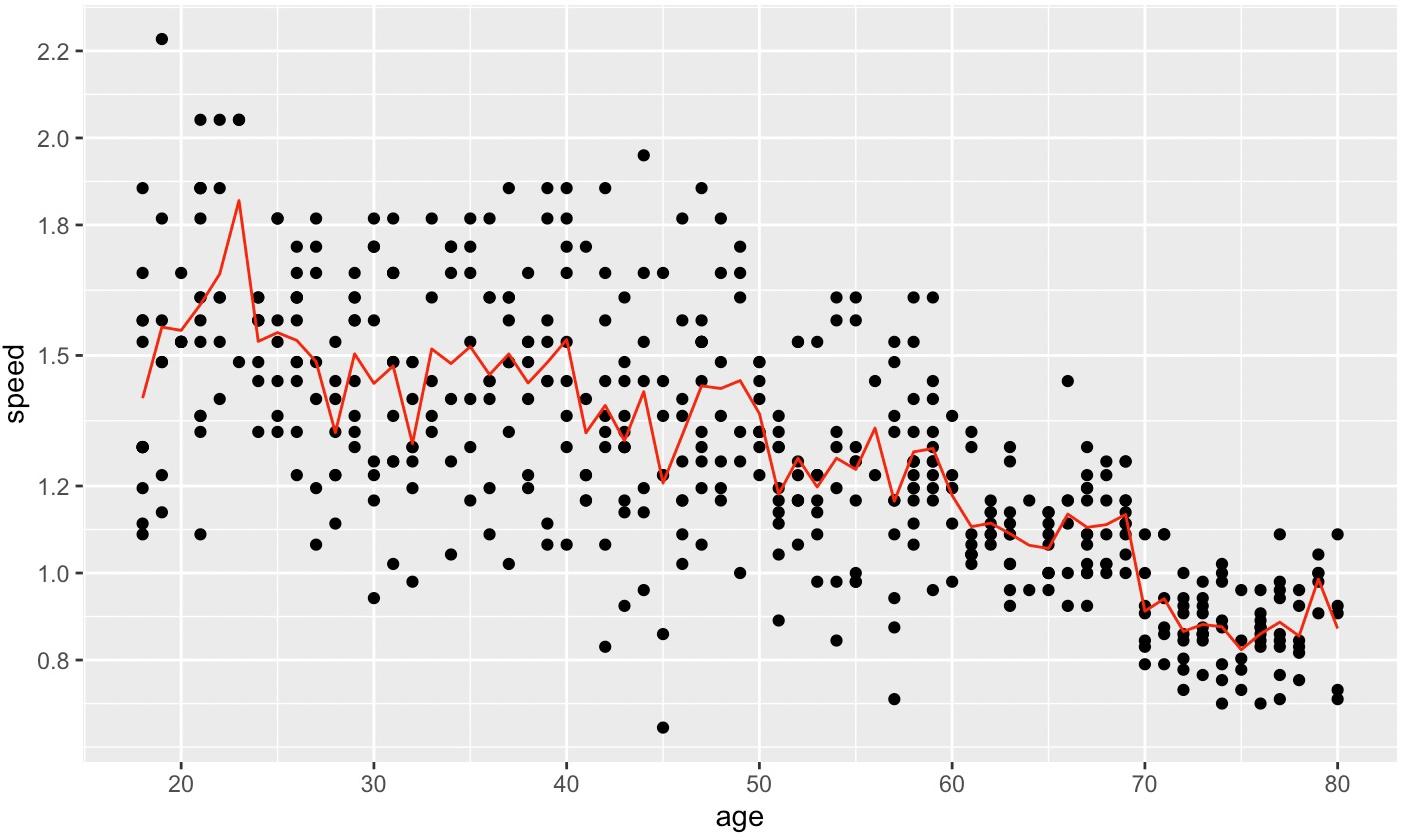
\includegraphics[width=0.5\textwidth]{images/plot500.jpg}}
 \caption{Scatter plots of the results of simulation of the scenario 7.}
 \label{scatter_plots}
\end{figure}

\begin{table}[H]\centering
    \csvreader[
      tabular=|c|c|c|c|,
      table head=\hline \bfseries{Id} & \bfseries{Age} & \bfseries{Expected speed} & \bfseries{Real speed}\\\hline,
      late after last line=\\\hline % horizontal line at the end of the table
    ]{pedestrian_records.csv}{}{\csvlinetotablerow}
    \caption[position=bottom]{Results of a simulation of the scenario 7}\label{pedestrian_recordings}
\end{table}

\end{task}

\begin{thebibliography}{9}
\bibitem{weidmann}
Weidmann U., Transporttechnik der Fußgänger, Schriftenreihe des Institut für Verkehrsplanung, Transporttechnik, Strassen- und Eisenbahnbau Nr. 90, S.35-46, Zürich, January 1992.
\bibitem{rimea}
RiMEA. Guideline for Microscopic Evacuation Analysis. RiMEA e.V., 3.0.0 edition, 2016. \url{www.rimea.de}.
\end{thebibliography}


\end{document}